\documentclass[a4paper, 12pt]{report}
% Allows writing the document in english.
\usepackage[utf8]{inputenc}
\usepackage[francais]{babel}
\usepackage[T1]{fontenc}
% Allows to use images.
\usepackage{graphicx}
% Provides hyperlinks within the document.
\usepackage{enumitem}
% Adds space between paragraphs.
\usepackage{parskip}
% Annexes
\usepackage{minitoc}
\usepackage{titletoc}
% Supports Text Companion fonts (necessary for gensymb).
\usepackage{textcomp}
\usepackage{array}
\usepackage{multicol}
% Better tabular
\usepackage{tabularx}
% Allows to use colors.
\usepackage{xcolor}
\usepackage[margin=4cm]{geometry}
\usepackage{varwidth}
% Euro
\usepackage{eurosym}
\usepackage{amsmath}

\usepackage{subfigure}
\usepackage[
    type={CC},
    modifier={by-nc-nd},
    version={4.0},
]{doclicense}

\usepackage[colorlinks=true,urlcolor=black,linkcolor=black]{hyperref}
% New columns types
% Left
\newcolumntype{L}{>{\raggedright\arraybackslash}X}
% Center
\newcolumntype{C}{>{\centering\arraybackslash}X}
% Right
\newcolumntype{R}{>{\raggedleft\arraybackslash}X}

% Add more space before and after table
\newenvironment{centerspace}{\setlength{\topsep}{1ex}\center}{\endcenter}
% Sets the color of gray.
\newcommand{\gray}{\rowcolor[gray]{.90}}
% Allows to draw lines.
\newcommand{\HRule}{\rule{\linewidth}{0.5mm}}
% Uses the arabic numerals for sections.
\renewcommand{\thesection}{\arabic{section}}

% Width of text.
\addtolength{\textwidth}{2cm}
% Odd page left margin.
\addtolength{\oddsidemargin}{-1cm}
% Height of main text.
\addtolength{\textheight}{2cm}
% Removes indentation.
\setlength\parindent{0pt}
% Indicates overflow words.
\setlength{\overfullrule}{10pt}
% Height of items.
\setitemize{itemsep=1em}

%%%%********************************************************************
% fancy quotes
\definecolor{quotemark}{gray}{0.7}
\makeatletter
\def\fquote{%
    \@ifnextchar[{\fquote@i}{\fquote@i[]}%]
           }%
\def\fquote@i[#1]{%
    \def\tempa{#1}%
    \@ifnextchar[{\fquote@ii}{\fquote@ii[]}%]
                 }%
\def\fquote@ii[#1]{%
    \def\tempb{#1}%
    \@ifnextchar[{\fquote@iii}{\fquote@iii[]}%]
                      }%
\def\fquote@iii[#1]{%
    \def\tempc{#1}%
    \vspace{1em}%
    \noindent%
    \begin{list}{}{%
         \setlength{\leftmargin}{0.1\textwidth}%
         \setlength{\rightmargin}{0.1\textwidth}%
                  }%
         \item[]%
         \begin{picture}(0,0)%
         \put(-15,-5){\makebox(0,0){\scalebox{3}{\textcolor{quotemark}{``}}}}%
         \end{picture}%
         \begingroup\itshape}%
 %%%%********************************************************************
 \def\endfquote{%
 \endgroup\par%
 \makebox[0pt][l]{%
 \hspace{0.8\textwidth}%
 \begin{picture}(0,0)(0,0)%
 \put(15,15){\makebox(0,0){%
 \scalebox{3}{\color{quotemark}''}}}%
 \end{picture}}%
 \ifx\tempa\empty%
 \else%
    \ifx\tempc\empty%
       \hfill\rule{100pt}{0.5pt}\\\mbox{}\hfill\tempa,\ \emph{\tempb}%
   \else%
       \hfill\rule{100pt}{0.5pt}\\\mbox{}\hfill\tempa,\ \emph{\tempb},\ \tempc%
   \fi\fi\par%
   \vspace{0.5em}%
 \end{list}%
 }%
 \makeatother

 %%%% ********************************************************************

% To divide the bibliography
\usepackage{splitbib}

% Starts roman numbering (trick to not numbering the first pages).
\pagenumbering{roman}

\begin{document}
    %\renewcommand{\bibname}{Références}
    \begin{center}
  
\includegraphics[scale=0.12]{textures/logo/heh_bw.pdf}

  \vspace{1cm}

  \textsc{\LARGE Projet} \\ [0.5cm]
  \textsc{\Large Réalisation d'un site en PHP} \\ [0.5cm]

  \textsc{\large 2\up{ème} Bachelier en Informatique} \\ [0.2cm]

  \begingroup
  \fontfamily{pag} \selectfont 

  \HRule \\ [0.4cm] {
    \huge Programmation web \\ [0.2cm] 
  }
  \HRule \\ [1.3cm]
  \endgroup
  \begin{minipage}[t]{0.4 \textwidth} 
    \begin{flushleft} 
      \large \emph{Auteur:} \\ 
      Alexandre \textsc{Ducobu}
    \end{flushleft} 
  \end{minipage}
  % 
  \begin{minipage}[t]{0.4 \textwidth}
    \begin{flushright} 
      \large \emph{Enseignants :} \\ 
      Antoine \textsc{Malaise} \\
      Fabrice \textsc{Scopel}
    \end{flushright} 
  \end{minipage}

  \vspace{1cm}

  
\includegraphics[scale=0.08]{textures/logo/technical_bw.pdf}

  \vspace{0.5cm}

  Année académique 2016 - 2017
\end{center}

\thispagestyle{empty}

    \newpage
    \newpage
\thispagestyle{empty}
\setcounter{page}{0}
\null
\newpage
    \begin{center}
  
\includegraphics[scale=0.12]{textures/logo/heh.pdf}

  \vspace{2cm}

  \textsc{\LARGE Projet ARS} \\ [0.5cm]
  \textsc{\Large Les différents systèmes d'exploitation} \\ [0.5cm]

  \textsc{\large 1er Bachelier en Informatique} \\ [0.2cm]
  \textsc{Groupe 5-8} \\

  \begingroup
  \fontfamily{pag} \selectfont 

  \HRule \\ [0.4cm] {
    \huge Architecture des Systèmes II \\ [0.2cm] 
  }
  (Laboratoire)
  \HRule \\ [1.3cm]
  \endgroup

  \begin{minipage}[t]{0.4 \textwidth} 
    \begin{flushleft} 
      \large \emph{Auteur:} \\ 
      Agozzino \textsc{Terencio} 
    \end{flushleft} 
  \end{minipage}
  % 
  \begin{minipage}[t]{0.4 \textwidth}
    \begin{flushright} 
      \large \emph{Auteur :} \\ 
      Ducobu \textsc{Alexandre} 
    \end{flushright} 
  \end{minipage}

  \vspace{0.5cm}

  \begin{minipage}[t]{0.4 \textwidth}
    \begin{center} 
      \large \emph{Enseignant:} \\ 
      Desmet \textsc{Erwin} 
    \end{center} 
  \end{minipage}

  \vspace{0.5cm}

  
\includegraphics[scale=0.08]{textures/logo/technical.pdf}

  \vspace{0.5cm}

  Année académique 2015 - 2016
\end{center}

\thispagestyle{empty}

    \newpage
    \newpage
\thispagestyle{empty}
\setcounter{page}{0}
\null
\newpage
    \newpage
    \mbox{~}
\vfill
Ce document est mis à disposition selon les termes de la licence Creative
Commons ``\href{https://creativecommons.org/licenses/by-nc-nd/4.0/}{Attribution -
Pas d'utilisation commerciale 4.0 International}''.

\begin{figure}[!h]
  \centering
  
\includegraphics[width=0.25\textwidth]
  {textures/images/license/license.eps}
\end{figure}

\thispagestyle{empty}

    \newpage
    \pagenumbering{arabic}
    \dominitoc
    \tableofcontents
    \newpage
    \section{Présentation du projet}
\label{sec:presentation}


\subsection{Introduction}
\label{subsec:intro}

Dans le cadre du cours de \textbf{Gestion de projets}, il nous a été demandé de réaliser un projet au choix individuellement ou par deux. J'ai choisi de le faire seul. \\
En effet, nous avons déjà d'autres travaux de groupes. Je trouve donc qu'un travail individuel est un plus dans notre cursus scolaire. \\
Lors des deux premières séances de laboratoire, chaque groupe a rédigé une fiche descriptive du projet, avec l’enseignant, afin de baliser le travail à effectuer durant l’année.\\
Lors de ces séances, l’enseignant a validé chacun des projets.


\subsection{But}
\label{subsec:but}

Grâce à ce projet, nous allons apprendre à gérer nos projets à l'aide de différents outils spécialisés tels que \textbf{\textit{Microsoft Project}}, \textit{le diagramme de \textbf{Gantt}} et \textit{le graphique de \textbf{PERT}}.\\
Ceux-ci nous aideront dans la planification de notre projet ainsi que, pour les binômes, dans la répartition des tâches. 


\subsection{Choix du projet}
\label{subsec:choix}

Ce projet, \textit{un site web}, permettra d'apprendre les bases de la programmation en \textit{Python} et sera divisé en chapitres: les variables, les conditions, les boucles, les tableaux, etc.\\

L’apprentissage se fera en trois étapes:
\begin{enumerate}
    \item L’utilisateur découvrira le nouveau sujet par de la théorie ainsi que par un ou plusieurs exemples. Il en apprendra alors l’utilité et le fonctionnement.
    \item Entre deux parties théoriques, l’utilisateur mettra en pratique ce qu’il aura appris au travers de petits QCM.
    \item Une fois le chapitre terminé, un questionnaire (QCM, ordonnancement du code,...) sera proposé à l’utilisateur.\\
    Celui-ci sera noté sur 10 afin que l’utilisateur puisse se juger et s’améliorer.\\
    Le passage au chapitre suivant requerra une \textit{cote minimale de 7/10}.\\
\end{enumerate}

D'autre part, ce projet sera un pré-TFE.\\
À terme, il sera possible de créer facilement des cours et de s’y inscrire.\\ Il pourra être utilisé aussi bien par les écoles que par  \og \textit{les particuliers} \fg.


%%% Local Variables:
%%% mode: latex
%%% TeX-master: t
%%% End:

    \newpage
    \section{État des lieux}
\label{sec:etat-lieux}


\subsection{Étapes de création}
\label{subsec:etapes-de-création}

Lors de la phase de préparation du site, j'ai débuté par la création de maquettes \textit{(voir\textbf{~\nameref{sec:maquettes}})} afin de partir sur une idée concrète du projet.\\

Je me suis ensuite engagé dans la phase d'écriture des chapitres et des questionnaires. \\
Le premier jet comptait trois chapitres (\textit{les variables, les booléens et la complexité}), dont le dernier était trop complexe pour débuter dans la programmation.\\
Il est resté à son état d'origine, et n'est donc pas disponible dans le site.\\

Après ces deux phases, est venue celle de la création du squelette du site en HTML et CSS, suivie de \textit{\textbf{très}} près par l'ajout des effets en JavaScript. \\

À ce moment, le projet a été mis en pause dans le but :
\begin{enumerate}

    \item de concevoir et de préparer la présentation du projet;
    \item d'étudier pendant le pré-blocus de Pâques;
    \item d'avancer dans les autres projets, dont celui du cours d'\textit{Initiation aux nano-ordinateurs} qui devait être achevé pour le 12 mai.\\
    
\end{enumerate}

La phase suivante a été l'une des plus importantes du projet : c'est la liaison du site à la base de données. \\
En effet, le site est désormais dynamique :
\begin{itemize}

    \item[$\bullet$] L'accès aux chapitres n'est plus permis que s'ils ont été débloqués dans la base de données;
    \item[$\bullet$] Les résultats obtenus à la fin des chapitres, et disponibles dans les trophées, proviennent aussi de la base de données.\\
    
\end{itemize}

La dernière phase - \textit{la phase de finalisation} - consiste à la réécriture des chapitres existants (\textit{les variables et les booléens}) ainsi qu'à l'écriture des autres chapitres (\textit{l'introduction, les conditions et les boucle}s) et à l'ajout des différents questionnaires. \\
Bien entendu, tout au long de cette période, le site a été testé de manière à ce qu'il soit le plus stable possible.

\newpage


\subsection{Choix des technologies}
\label{subsec:choix-des-technologies}

Vu la nature du projet, \textit{un site web dynamique}\footnote{Un site dynamique est un site dont les données proviennent d’une base de données.}, j'ai utilisé les langages suivants :
\begin{itemize}

    \item[$\bullet$] le HTML et le CSS pour la création du site;
    \item[$\bullet$] le JavaScript (\textit{et le jQuery}) pour l'ajout d'animations et d'effets;
    \item[$\bullet$] le PHP et le MySQL pour la connexion au site et l'accès à la base de données. \\

\end{itemize}

Pendant les premières phases du projet, l'éventualité d'utiliser \textit{Bootstrap} et le framework PHP \textit{Laravel} est apparue. \\

\textbf{Bootstrap} est une collection d'outils utile à la création du design de sites et d'applications web [\textit{sic}]\footnote{\url{https://fr.wikipedia.org/wiki/Bootstrap_(framework)}}. \\
Ces outils - \textit{composés de codes HTML et CSS} - permettent d'utiliser facilement des formulaires, des boutons, etc. \\
Ils facilitent aussi la conception de sites web adaptatifs grâce à la décomposition du site en colonnes. \\

Un framework évite de réinventer la roue en réutilisant ce qui a déjà été fait, utilisé et validé par de nombreux utilisateurs. \\
Cela représente, donc, un gain de temps, de fiabilité et une facilité de mise à jour. \\
\textbf{Laravel} regroupe aussi de nombreuses bibliothèques qui facilitent la gestion des sessions, l’authentification, un créateur de requêtes SQL,... \\

Mais il y a un mais : pour les utiliser, il faut se documenter, apprendre et expérimenter, ce qui représente beaucoup de temps. Trop par rapport à celui que je possédais.

Je ne les ai donc pas utilisés, mais j'ajouterai que la non utilisation de ces outils permet plus de libertés et de personnalisation du site.


%%% Local Variables:
%%% mode: latex
%%% TeX-master: t
%%% End:
    \newpage
    \section{Diagrammes}
\label{sec:diagrammes}

Afin de gérer le projet, j'ai utilisé plusieurs logiciels. \\

Pour la création du diagramme de \textbf{Gantt}, j'ai d'abord employé \textit{GanttProject} qui ne m'a pas permis d'avoir deux tâches décallées en parallèle. Je me suis alors tourné vers \textit{Microsoft Project} qui, lui, m'a donné satisfaction. \\

Quant à celui de \textbf{PERT}, je l'ai conçu \textit{à la main}, car aucun outil ne proposait de concevoir le diagramme selon les instructions données dans le cours.

\newpage


\subsection{Gantt}
\label{subsec:gantt}

Voici le diagramme de Gantt du projet et son tableau descriptif :

%\vspace{0.5cm}

\begin{figure}[!h]
    \centering
    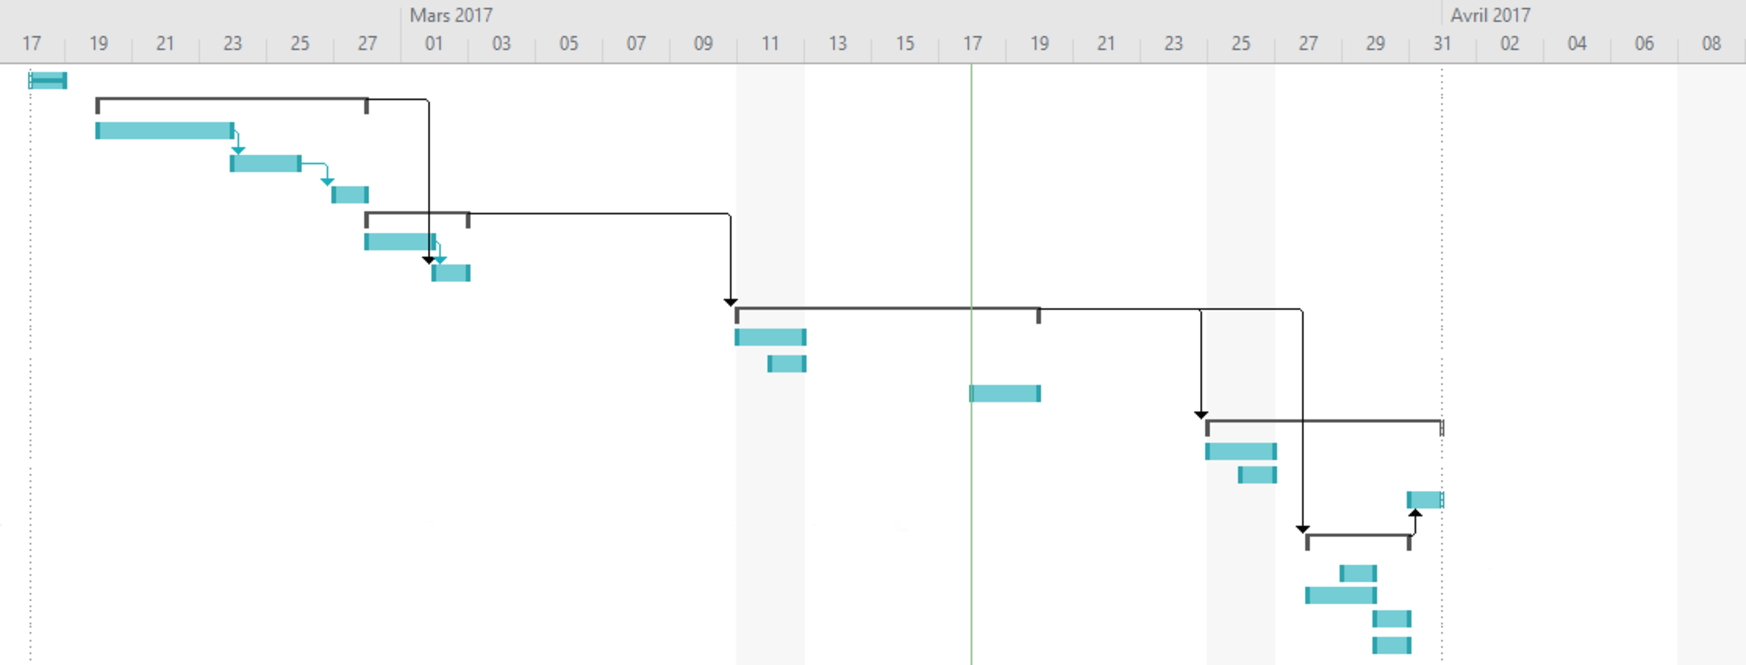
\includegraphics[scale=0.5]{textures/images/diagrammes/DiagrammeDeGantt.pdf}
    \caption{Diagramme de Gantt}
\end{figure}
\begin{figure}[!h]
    \centering
    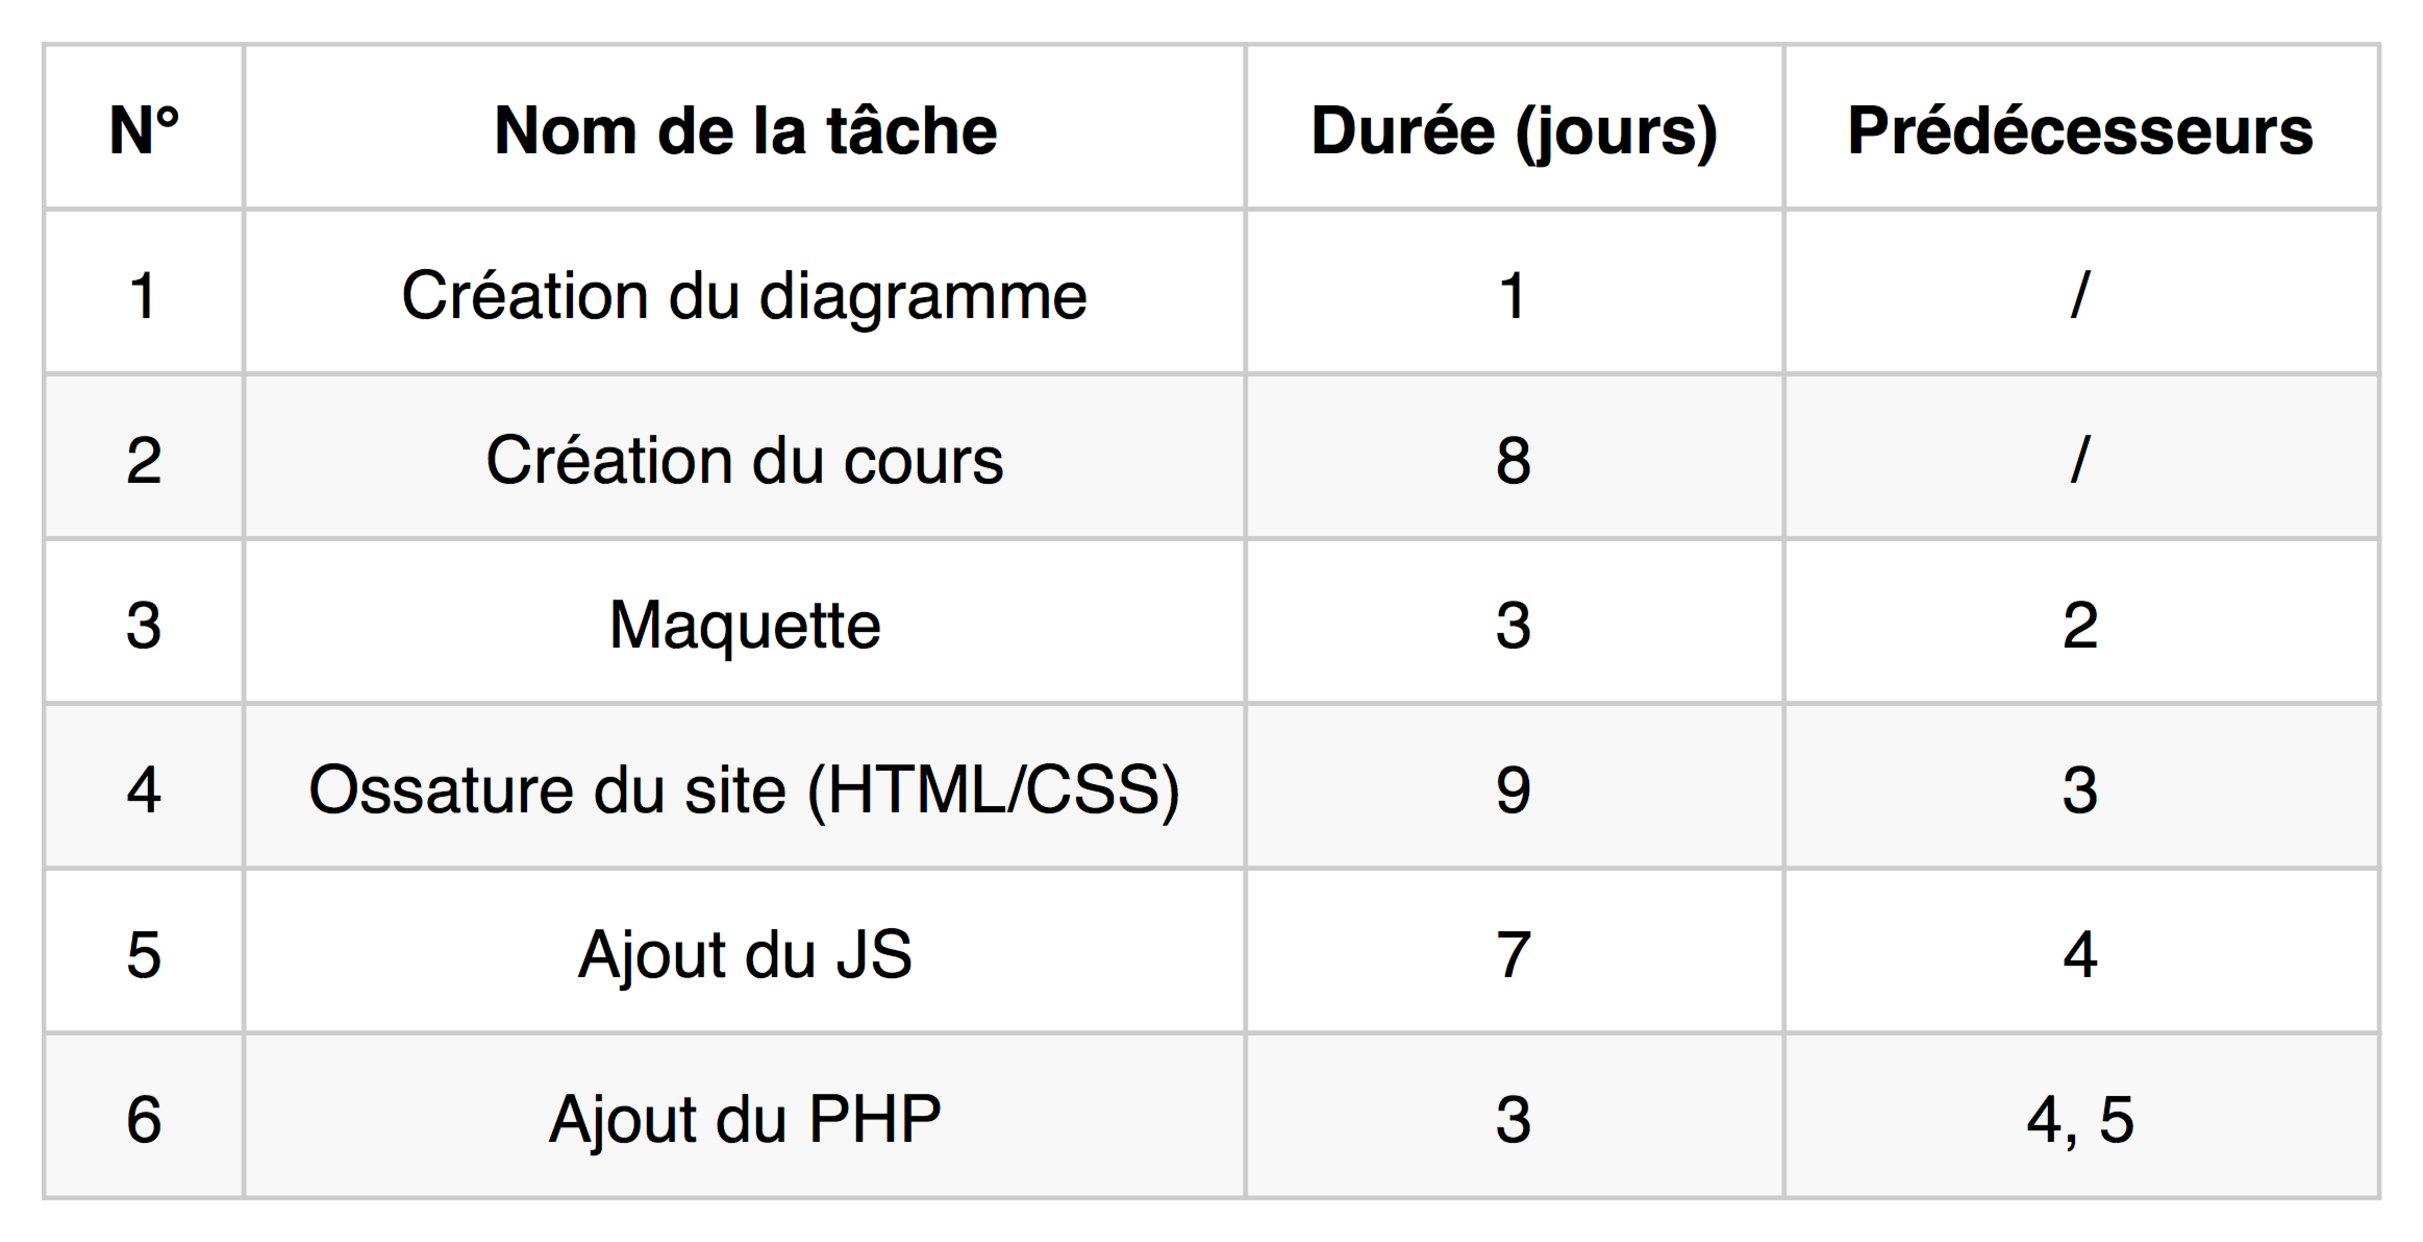
\includegraphics[scale=0.3]{textures/images/diagrammes/TableauDeGantt_brief.pdf}
    \caption{Tableau descriptif}
\end{figure}

Comme on peut le voir, la durée totale prévue du projet est de 31 jours.\\

Le projet est découpé en 6 tâches principales détaillées ci-dessous. \\

La création du diagramme a duré moins d'un jour, mais c'était la durée minimale disponible dans \textit{Microsoft Project}… \\

\newpage

La création du cours comprend l'écriture des différents chapitres et questionnaires. \\
Comme dit précédemment, celle-ci s'est déroulée en deux étapes :
\begin{enumerate}

    \item L'écriture d'un premier jet de trois chapitres : les variables, les booléens et la complexité, et… de quelques exercices.
    \item La réécriture des chapitres sur les variables et les booléens, et l'écriture des autres chapitres \textit{(l'introduction, les conditions et les boucles)}. Chacun accompagné de son questionnaire principal et de ses questionnaires secondaires. \\
    Le questionnaire principal teste, en quatre questions, les connaissances acquises tout au long du chapitre, tandis que les secondaires testent celles de la page précédente en deux questions.\\
    
\end{enumerate}

Cinq maquettes ont été créées :
\begin{enumerate}

    \item La page d'accueil, très \textit{(trop)} simple et sobre;
    \item La page du cours comprenant les liens vers les chapitres;
    \item L'aperçu d'un chapitre. C'est la raison pour laquelle les maquettes dépendent de la tâche précédente;
    \item La page des trophées;
    \item La page du compte de l'utilisateur. \\
    
\end{enumerate}

Dans la version finale, on peut remarquer que le design a évolué. Comme lors d'une démonstration, celui-ci a été jugé \og \textit{trop simple} \fg j'en ai profité pour ajouter des \textbf{animations} sur la page d’accueil, sur les chapitres ainsi que sur les trophées, et de la \textbf{coloration syntaxique} du code. \\

La création de l'ossature du site fut la partie la plus longue parce que la majorité du code du site a été écrite à ce moment. \\
Ainsi, toutes les pages \textit{(accueil, cours, chapitres, trophées, etc.)}, styles et effets CSS ont été créés et n'ont plus été changés depuis. \\

L'ajout du JavaScript est autant lié au code HTML qu'à celui en PHP : il est utilisé dans tout ce qui est animations et boutons. \\
Par exemple, les boutons utilisés pour modifier les données de l'utilisateur ou pour supprimer le compte sont écrits en HTML et CSS. L'action est exécutée en JavaScript et passe par le PHP pour se connecter à la base de données. \\

Pour terminer, l'ajout du PHP a été un gros morceau : le fait de mixer les codes HTML, PHP et MySQL n'a pas été simple. \\
En effet, comme c'est mon premier projet, \textit{en parallèle avec celui du cours de PHP}, à mettre en œuvre un site connecté à une base de données, cela m'a demandé pas mal de travail pour arriver au bon résultat. \\
De plus, sans le PHP, il n'y aurait pas de connexion, d'inscription ou de déblocage des chapitres. Tout cela est directement lié à la base de données, elle-même liée au site par le PHP.

\newpage


\subsection{PERT}
\label{subsec:pert}

Après avoir travaillé le diagramme de Gantt, j'ai réalisé le diagramme de PERT.
Ci-dessous, vous pouvez le voir dans sa forme initiale :

\begin{figure}[h]
  \centering
  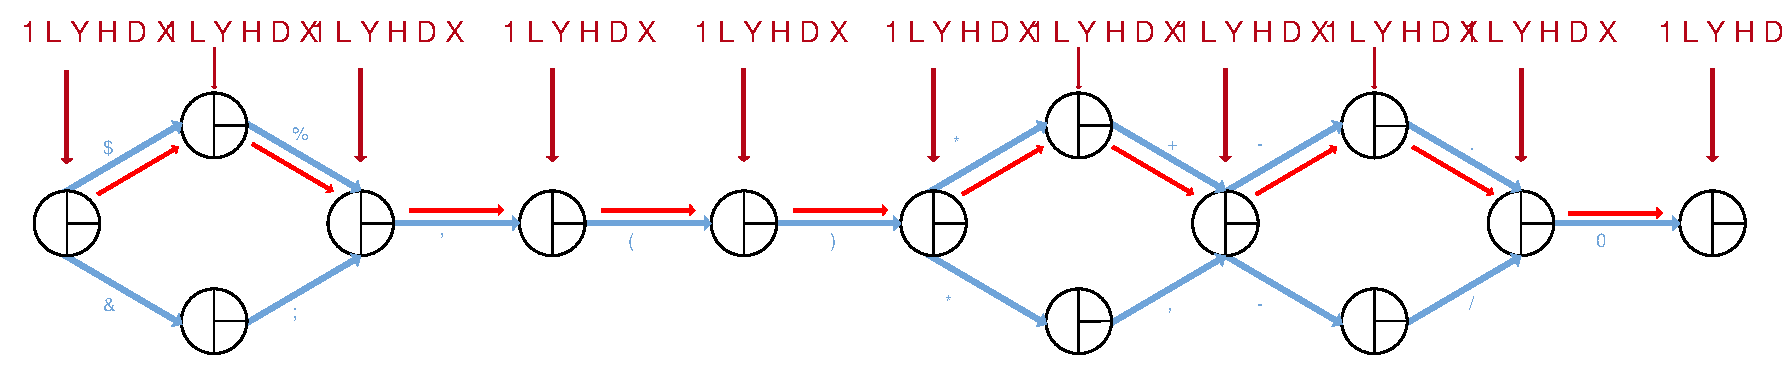
\includegraphics[scale=0.49]
  {textures/images/diagrammes/DiagrammeDePert1.pdf}
  \caption{Diagramme de PERT initial}
  \label{fig:pert-initial}
\end{figure}

Après que le projet soit terminé, j'ai refait le diagramme de PERT afin de coller au plus près au temps passé sur les différentes tâches :

\begin{figure}[h]
  \centering
  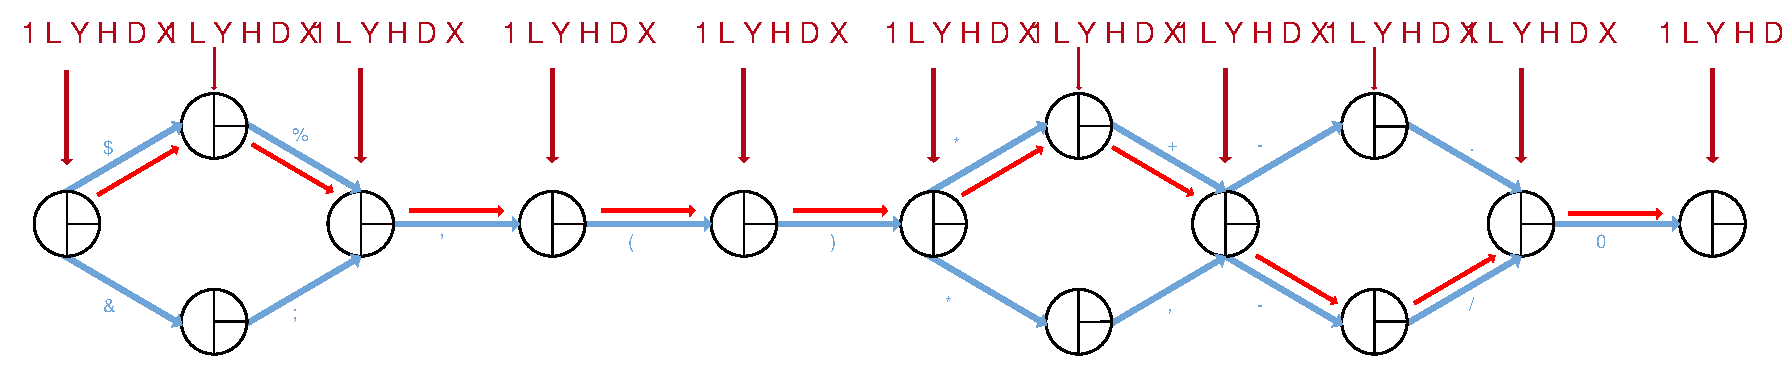
\includegraphics[scale=0.49]
  {textures/images/diagrammes/DiagrammeDePert2.pdf}
  \caption{Diagramme de PERT final}
  \label{fig:pert-final}
\end{figure}

La première chose que l'on peut remarquer, c'est qu'il a fallu moins de temps que prévu pour terminer le projet \textit{(on passe de \textbf{29h15} à \textbf{27h})}. \\

Dans ce diagramme, les tâches sont plus nombreuses pour plus de précision, et leur durée est plus juste. On parle désormais en heures et plus en jours. \\
Par exemple, on peut voir que l'écriture des chapitres dure 8 heures et que celle des exercices en dépend. \\
De même pour la création de la maquette qui ne dépend plus entièrement des tâches ci-dessus. C'est la tâche \textbf{D}, le test de la maquette avec le texte, qui dépend de l'existence du cours, et elle ne dure qu'un quart d'heure.

\newpage

Voici le tableau des antériorités lié au diagramme final :

\begin{figure}[h]
  \centering
  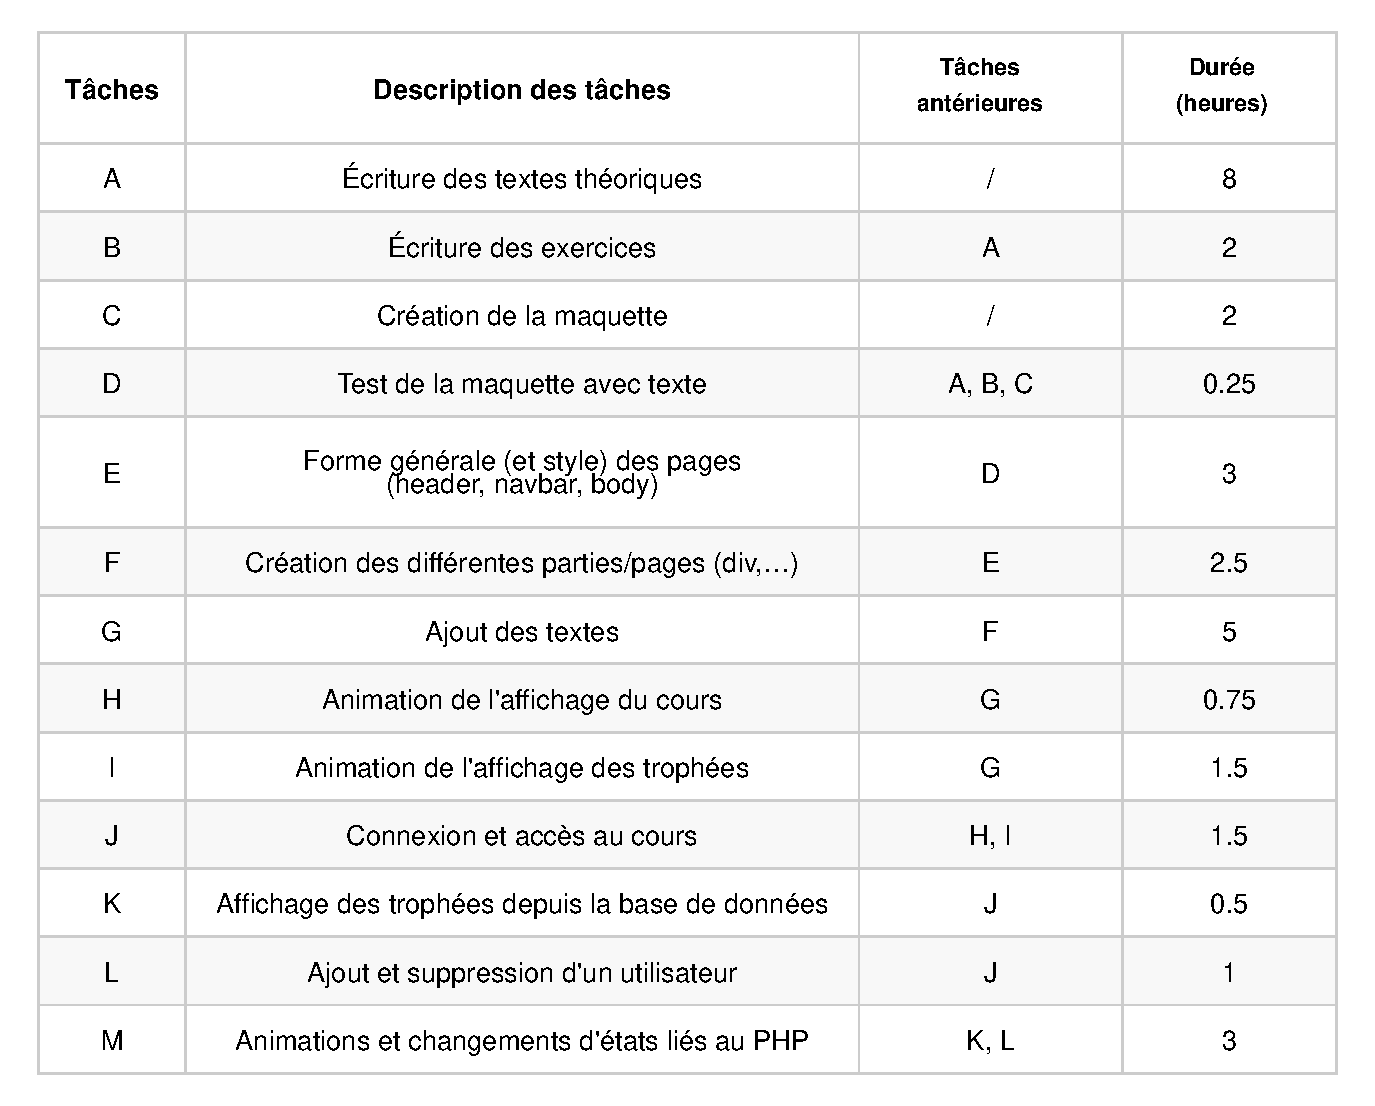
\includegraphics[scale=0.6]
  {textures/images/diagrammes/TableauDesAnteriorites.pdf}
  \caption{Tableau des antériorités}
  \label{fig:tableau-anteriorites}
\end{figure}


{\Large \textbf{Différences entre l'initial et le final}}

Jusqu'à la tâche \textbf{F}, \textit{niveau 7}, il n'y a pas de différences. \\
Après celle-ci, quatre des sept tâches ont eu des durées différentes de ce que j'avais escompté :

\begin{enumerate}

    \item la tâche \textbf{G} est passée de \textbf{1h30} à \textbf{5h}. La cause est simple, la mise en page des chapitres a été plus complexe que prévu.
    En cause, l'ajout de coloration syntaxique, l'ajout de styles pour les types \textit{(gras, italique, etc.)}, ainsi que l'ajout d'un slider \footnote{\url{http://callmenick.com/post/responsive-content-slider}} divisant les chapitres en différentes parties, etc.
    
    \item la connexion à la base de données, tâche \textbf{J}, a pris moins de temps que prévu. \\
    \textbf{Remarquons}, tout de même, que de nombreux changements à ce niveau ont été effectués à la tâche \textbf{M}, dont la raison d'être était de résoudre les problèmes potentiels.
    
    \item l'affichage du résultat dans les trophées \textit{depuis la base de données}, \textit{la tâche \textbf{K}}, a été beaucoup moins difficile qu'imaginé grâce à l'avancée du projet du cours de \textit{Programmation web}.
    
    \item il en est de même pour la tâche \textbf{L}, \textit{l'ajout et la suppression d'utilisateurs}, a donc pris moins de temps.

\end{enumerate}

%%% Local Variables:
%%% mode: latex
%%% TeX-master: t
%%% End:

    \newpage
    \section{Base de données}
\label{sec:BD}


\subsection{Création de la base de données}
\label{subsec:creation-db}

La base de données est composée de huit tables contenant toutes les données utiles au bon fonctionnement du site. \\

Les six tables de la figure~\ref{fig:db2} ont été créées en plus de celles ajoutées par Laravel\footnote{La table \textbf{users} a été créée par Laravel, mais modifiée afin de répondre aux besoins du site.}. \\
Il y a la table :
\begin{itemize}
    
    \item \textbf{users} qui contient tout ce qui concerne les utilisateurs;
    
    \item \textbf{comments} qui contient la liste des commentaires;
    
    \item \textbf{courses} qui contient les informations des cours;
    
    \item \textbf{chapters} qui contient les chapitres;
    
    \item \textbf{enrollments} qui contient la liste des inscriptions aux cours;
    
    \item \textbf{tests} qui contient les tests.
    
\end{itemize} 

\vspace{0.5cm}

\begin{figure}[h]
  \centering
  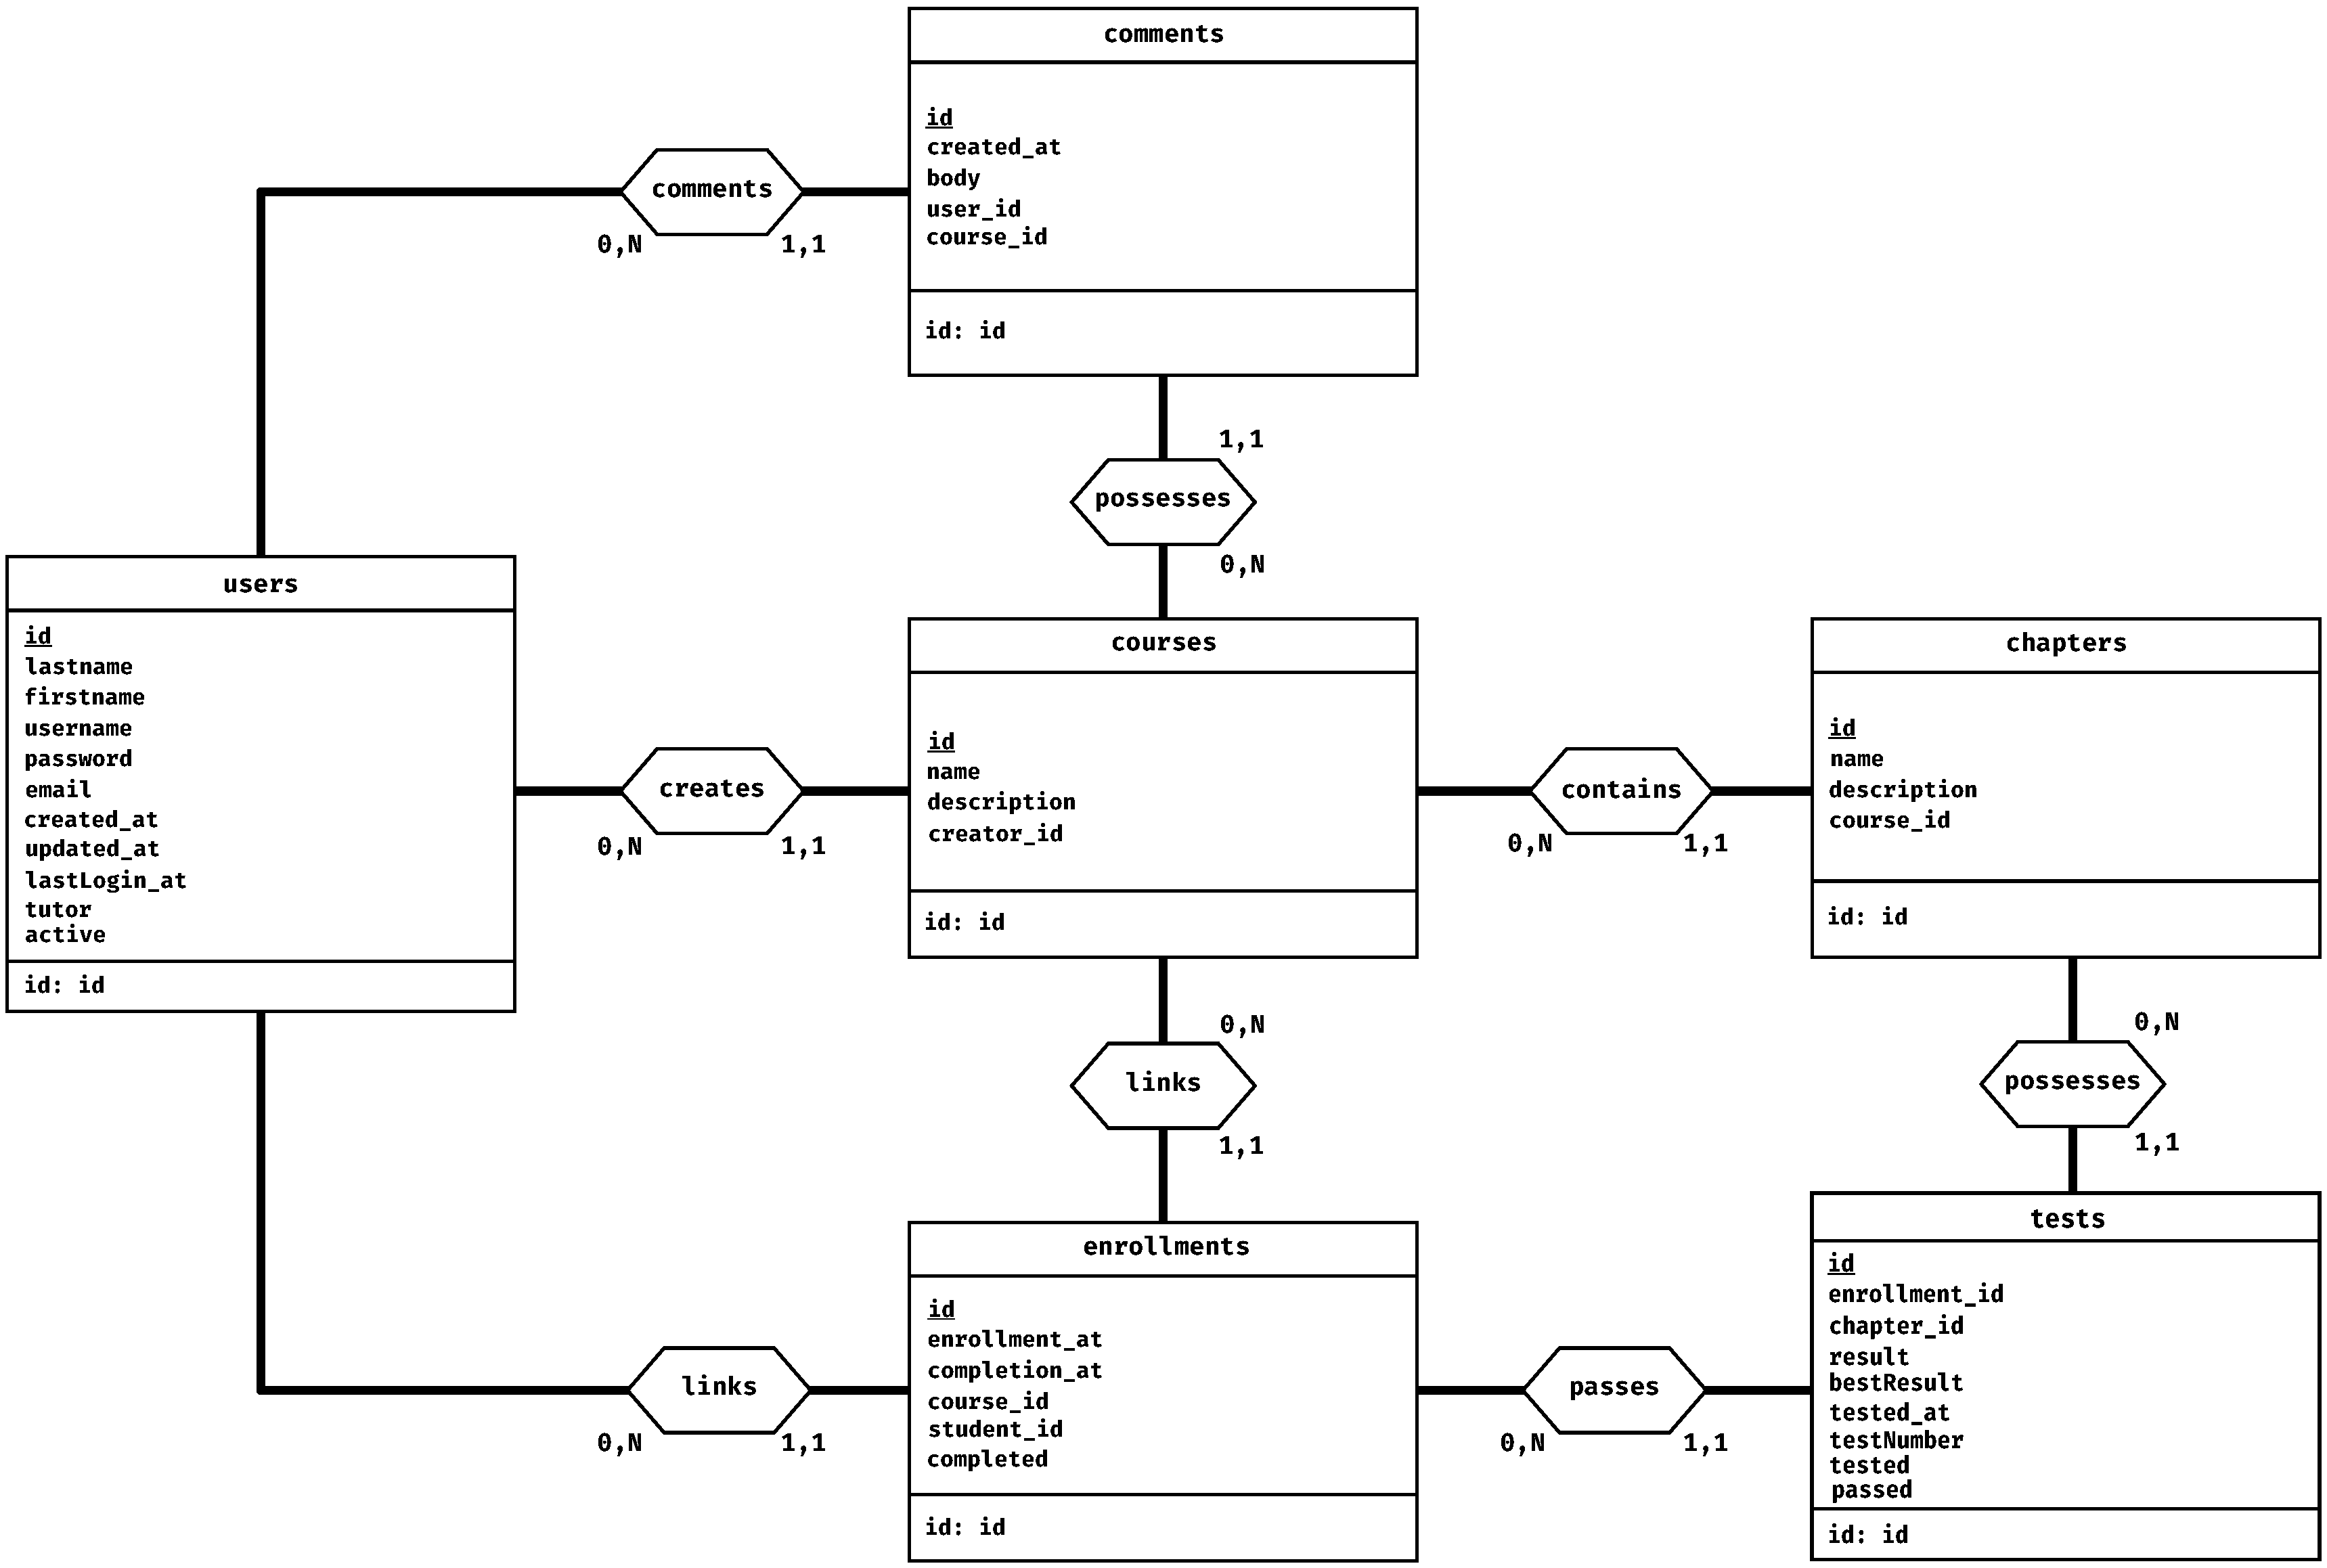
\includegraphics[width=\textwidth]
  {textures/images/DB/Student-Tutor.pdf}
  %\caption[Figure 1]{Schéma conceptuel de la base de données}
  \caption{Schéma conceptuel de la base de données}
  \label{fig:db2}
\end{figure}

\newpage

Le framework Laravel a donc créé trois tables dont \textbf{users}.\\
Les deux autres tables sont \textbf{migrations} et \textbf{password\_resets}.\\
La première gère les migrations \textit{(par exemple : la création des différentes tables)}. \\
La seconde gère la réinitialisation des mots de passe.

\vspace{0.5cm}

\begin{figure}[h]
  \centering
  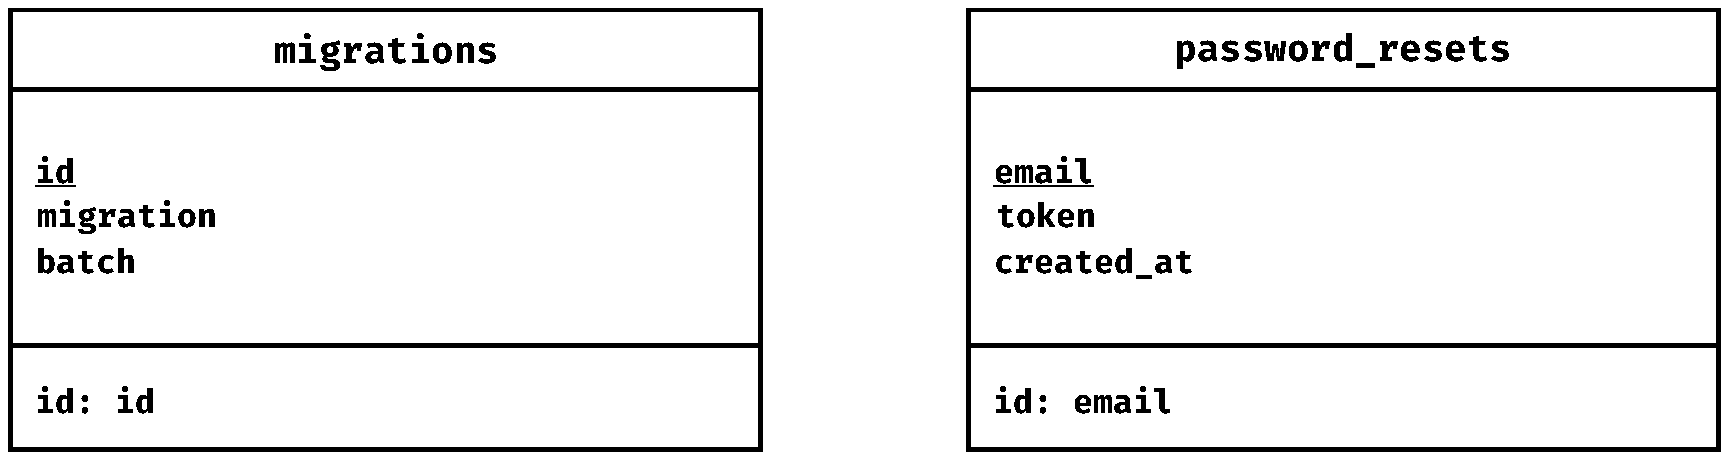
\includegraphics[width=\textwidth]
  {textures/images/DB/Other-Laravel.pdf}
  \caption{Tables créées par Laravel}
  \label{fig:db1}
\end{figure}

\vspace{0.5cm}


\newpage


\subsection{Vue détaillée}
\label{sec:vue-details}
Dans cette section, chaque table sera décrite ainsi que son fonctionnement.


\subsubsection{Table \textit{users}}
\label{sec:table-users}
C'est la table contenant les données de chaque utilisateur et l'état de leur compte.\\
Un utilisateur peut s'inscrire à des cours ou écrire des commentaires et des cours.

Les différents champs sont :

\begin{itemize}
    
    \item[$\bullet$] \textbf{id} est l'identifiant unique de l'utilisateur.\\
    Il sert de clé primaire à la table et est auto-incrémenté à partir de un.
    
    \item[$\bullet$] \textbf{lastname} est le nom de famille de l'utilisateur.
    
    \item[$\bullet$] \textbf{firstname} est le prénom de l'utilisateur.
    
    \item[$\bullet$] \textbf{username} est le nom d'utilisateur unique choisi lors de l'inscription.
    
    \item[$\bullet$] \textbf{password} est le mot de passe de l'utilisateur. Il a une taille minimale de 6 caractères, pouvant être composé de caractères alphanumériques, de tirets et de tirets bas \textit{(underscore)}.\\
    Celui-ci est haché \footnote{\href{https://fr.wikipedia.org/wiki/Fonction\_de\_hachage\_cryptographique}{Wikipédia, Fonction de hachage cryptographique :  https://fr.wikipedia.org/wiki/Hachage}} à l'aide de \textit{Bcrypt} qui est une fonction de hachage incluse dans Laravel.
    
    \item[$\bullet$] \textbf{email} contient l'adresse mail de l'utilisateur.\\
    Ce champ est unique, vu qu'il sert à la connexion de l'utilisateur.
    
    \item[$\bullet$] \textbf{created\_at} contient la date et l'heure de création de l'utilisateur.
    
    \item[$\bullet$] \textbf{updated\_at} contient la date et l'heure de modification de l'utilisateur.
    
    \item[$\bullet$] \textbf{lastLogin\_at} contient la date et l'heure de la dernière connexion de l'utilisateur.
    
    \item[$\bullet$] \textbf{tutor} indique si l'utilisateur a déjà un ou plusieurs cours \textit{(valeur à 1)}, sinon ce sera la valeur par défaut \textit{(valeur à 0)}.
    
    \item[$\bullet$] \textbf{active} donne l'état du compte de l'utilisateur:
    
    \begin{itemize}
        
        \item \textbf{0} indique que le compte est inactif.\\
        Cela signifie que le compte a été supprimé ou que l'administrateur a banni l'utilisateur.
        
        \item \textbf{1} indique que le compte est actif \textit{(par défaut)}.
        
    \end{itemize}
    
\end{itemize}


\newpage


\subsubsection{Table \textit{comments}}
\label{sec:table-comments}
C'est la table contenant les différents commentaires.\\
Ceux-ci sont liés à un utilisateur et à un cours.

Les différents champs sont :

\begin{itemize}
    
    \item[$\bullet$] \textbf{id} est l'identifiant unique du commentaire.\\
    Il sert de clé primaire à la table et est auto-incrémenté à partir de un.
    
    \item[$\bullet$] \textbf{created\_at} contient la date et l'heure de création du commentaire.
    
    \item[$\bullet$] \textbf{body} contient le corps du commentaire.
    
    \item[$\bullet$] \textbf{user\_id} est l'identifiant de l'utilisateur qui l'a écrit.
    
    \item[$\bullet$] \textbf{course\_id} indique le cours auquel le commentaire est lié.
    
\end{itemize}


\subsubsection{Table \textit{courses}}
\label{sec:table-courses}
C'est la table contenant les différents cours.\\
Ceux-ci sont liés à un utilisateur \textit{(son auteur)}, des commentaires et des inscriptions \textit{(enrollments)}.

Les différents champs sont :

\begin{itemize}
    
    \item[$\bullet$] \textbf{id} est l'identifiant unique du cours.\\
    Il sert de clé primaire à la table et est auto-incrémenté à partir de un.
    
    \item[$\bullet$] \textbf{name} est le nom unique du cours.
    
    \item[$\bullet$] \textbf{description} contient la description du cours.
    
    \item[$\bullet$] \textbf{creator\_id} est l'identifiant de l'utilisateur qui l'a écrit.
    
\end{itemize}

\newpage

\subsubsection{Table \textit{chapters}}
\label{sec:table-chapters}
Cette table contient les différents chapitres.\\
Ils sont liés à un cours et à un test.

Les différents champs sont :

\begin{itemize}
    
    \item[$\bullet$] \textbf{id} est l'identifiant unique du chapitre.\\
    Il sert de clé primaire à la table et est auto-incrémenté à partir de un.
    
    \item[$\bullet$] \textbf{name} est le nom du cours.
    
    \item[$\bullet$] \textbf{description} contient la description du chapitre.
    
    \item[$\bullet$] \textbf{course\_id} est l'identifiant du cours auquel il appartient.
    
\end{itemize}


\subsubsection{Table \textit{enrollments}}
\label{sec:table-enrollments}
Cette table contient les différentes inscriptions aux cours.\\
Ils sont liés à un cours, un utilisateur \textit{(celui qui est inscrit)} et à un test.

Les différents champs sont :

\begin{itemize}
    
    \item[$\bullet$] \textbf{id} est l'identifiant unique de l'inscription.\\
    Il sert de clé primaire à la table et est auto-incrémenté à partir de un.
    
    \item[$\bullet$] \textbf{enrollments\_at} contient la date et l'heure d'inscription au cours.
    
    \item[$\bullet$] \textbf{completion\_at} contient la date et l'heure d'achèvement du cours.
    
    \item[$\bullet$] \textbf{course\_id} est l'identifiant du cours auquel l'utilisateur est inscrit.
    
    \item[$\bullet$] \textbf{student\_id} est l'identifiant d'utilisateur inscrit.
    
    \item[$\bullet$] \textbf{completed} donne l'état de l'achèvement du cours :
    
    \begin{itemize}
        
        \item \textbf{0} indique que l'utilisateur n'a pas encore achevé le cours \textit{(par défaut)}.
        
        \item \textbf{1} indique que l'utilisateur a achevé le cours.
        
    \end{itemize}
    
\end{itemize}

\newpage

\subsubsection{Table \textit{tests}}
\label{sec:table-tests}
Cette table contient les différents tests.\\
Ils sont liés à un chapitre et à une inscription.

Les différents champs sont :

\begin{itemize}
    
    \item[$\bullet$] \textbf{id} est l'identifiant unique du test.\\
    Il sert de clé primaire à la table et est auto-incrémenté à partir de un.
    
    \item[$\bullet$] \textbf{enrollment\_id} est le nom du cours.
    
    \item[$\bullet$] \textbf{chapter\_id} est l'identifiant du chapitre auquel il est lié.
    
    \item[$\bullet$] \textbf{result} est le dernier résultat obtenu.
    
    \item[$\bullet$] \textbf{bestResult} est le meilleur résultat obtenu.
    
    \item[$\bullet$] \textbf{tested\_at} contient la date et l'heure du dernier test.
    
    \item[$\bullet$] \textbf{tested} indique si le test a déjà été passé :
    
    \begin{itemize}
        
        \item \textbf{0} l'utilisateur n'a pas encore passé le test \textit{(par défaut)}.
        
        \item \textbf{1} le test a été passé.
        
    \end{itemize}
    
    \item[$\bullet$] \textbf{testNumber} indique combien de fois le test a été passé par l'utilisateur.
    
    \item[$\bullet$] \textbf{passed} indique si le test a déjà été réussi :
    
    \begin{itemize}
        
        \item \textbf{0} l'utilisateur n'a pas encore réussi le test \textit{(par défaut)}.
        
        \item \textbf{1} le test a été réussi.
        
    \end{itemize}
    
\end{itemize}

\newpage

\subsubsection{Table \textit{migrations}}
\label{sec:table-migrations}
Cette table tient un historique des migrations.\\
Les migrations sont utilisées pour créer et définir des bases de données depuis des fichiers \textit{PHP} \textit{(cf. sous-section~\ref{subsec:migration} page~\pageref{subsec:migration})}. 


Les différents champs sont :

\begin{itemize}
    
    \item[$\bullet$] \textbf{id} est l'identifiant unique de la table.\\
    Il sert de clé primaire à la table et est auto-incrémenté à partir de un.
    
    \item[$\bullet$] \textbf{migration} est le nom du fichier \textit{PHP} créant la table.
    
    \item[$\bullet$] \textbf{batch} identifie la migration à laquelle la table a été créée \textit{(1 pour la première)}.
    
\end{itemize}


\subsubsection{Table \textit{password\_resets}}
\label{sec:table-password-resets}
Cette table permet de gérer la réinitialisation des mots de passe en toute sécurité.

Les différents champs sont :

\begin{itemize}
    
    \item[$\bullet$] \textbf{email} est l'identifiant unique de la réinitialisation, l'adresse mail de l'utilisateur qui réinitialise son mot de passe.
    
    \item[$\bullet$] \textbf{token} est le jeton de réinitialisation .
    
    \item[$\bullet$] \textbf{created\_at} contient la date et l'heure de création du jeton de réinitialisation.
    
\end{itemize}

\newpage

\subsection{Sécurité}
\label{subsec:securite}

\subsubsection{Injections SQL}
\label{sec:injections-sql}
Laravel fournit une méthode de protection contre les injections SQL. \\
Celles-ci forment l'une des méthodes d'attaque la plus connue et les plus dangereuses en PHP. \\
Les risques que représente ce genre de faille sont énormes : comme son nom l'indique, cette faille se manifeste lorsqu'il est possible d'injecter ou de modifier une requête SQL. \\
Ceci en injectant des morceaux de code \textit{non filtrés}, généralement par le biais d'un formulaire d'une page du site.

Le constructeur de requête \textit{(Query builder)} de Laravel utilise des instructions préparées de SQL qui rendent les attaques par injection inimaginables. \\
Il n'y a donc pas besoin d'effectuer de traitements sur les données avant de les passer au constructeur de requête. \\
Par contre, les requêtes brutes, utilisées en passant par \textit{DB::raw()}, y sont vulnérables vu que non préparées...

\subsubsection{Attaques CSRF}
\label{sec:attaques-csrf}
Le CSRF, ou Cross Site Request Forgery, est un type de vulnérabilité des services d'authentification web.\\
Le fonctionnement de l'attaque est simple : l'attaquant transmet une requête HTTP falsifiée à un utilisateur authentifié. Celle-ci pointe sur une action interne au site et est exécutée par l'utilisateur authentifié \textit{à son insu} et en utilisant \textit{ses propres droits}.

Une des possibilités de prévention est disponible dans Laravel : l'insertion de jetons de validité dans les formulaires.\\
Un formulaire posté n'est alors accepté que s'il a été produit quelques minutes auparavant : le jeton de validité en sera la preuve. Ce dernier doit être transmis en paramètre et vérifié côté serveur\footnote{\href{https://fr.wikipedia.org/wiki/CSRF}{Wikipédia, Cross-Site Request Forgery :  https://fr.wikipedia.org/wiki/CSRF}}.

    \newpage
    \section{Conclusion}
\label{sec:conclusion}


\subsection{Résultat}
\label{sec:resultat}

L'automate trie les boites d'après leur couleur \textit{(argent, cuivre et or)}.\\

Lorsqu'il est à l'arrêt, la lampe \textit{Hors-service} est allumée, et la lampe \textit{En service} est éteinte. \\

L'appui sur le bouton poussoir  \guillemotleft \ \textbf{Start} \guillemotright \ allume la lampe \textit{En service}, éteint la lampe \textit{Hors-service} et met en route le moteur du convoyeur principal.\\
Sauf dans le cas où un défaut moteur a été détecté, ce qui arrêterait \textit{totalement} le fonctionnement de l'automate.\\
Celui-ci devra d'abord être corrigé afin de désactiver l'alarme lumineuse par un acquittement à l'aide du sélecteur à clé \textbf{I16}. Le moteur pourra alors être mis en route.\\

Pour mettre en marche le moteur des convoyeurs d'évacuation, le sélecteur \textbf{I17} doit être enclenché.\\
S'il n'est pas enclenché, un défaut moteur sera levé et affiché par la lampe \textbf{Q1}. Voici les différents cas qui lèveront le défaut :

\begin{itemize}
    
    \item le cas du défaut au moteur principal, c'est le cas le plus simple.\\
    Le moteur se retrouve en surcharge, ce qui enclenche l'arrêt d'urgence.
    
    \item le cas du défaut au moteur des convoyeurs d'évacuation, divisé en différents cas.
    
    \begin{itemize}
    
        \item le cas simple, le moteur est en surcharge, ce qui enclenche l'arrêt d'urgence.
        
        \item le cas de l'encombrement des tapis d’évacuation.\\
        Il est levé lorsqu'une boite est sous le détecteur du tapis d'évacuation, et qu'une autre \textit{(du même type)} se retrouve devant le vérin.\\
        C'est le cas lorsque le moteur des tapis d’évacuation est à l'arrêt.
        
        \item le cas \textit{bonus}, les tapis d'évacuation sont stoppés, mais le moteur principal ne l'est pas.\\
        Lorsqu'une boite est détectée par le dernier détecteur, \textbf{I3}, un défaut est levé.\\
        Sans ce dernier cas, la boite tomberait du tapis.
        
    \end{itemize}
    
\end{itemize}

\newpage

Lorsqu'une boite argentée ou cuivrée est repérée par le détecteur idoine, le moteur principal s'arrête et le vérin place la boite sur le tapis d'évacuation approprié.\\
Le vérin se replace et le moteur principal se relance une fois que la boite est détectée sur son tapis d'évacuation.\\
À ce moment, le compteur qui lui est lié s'incrémente de un.\\

Pour les boites dorées, il n'y a pas de vérin, donc pas d'arrêt du moteur principal.\\
En effet, une fois arrivées au bout du tapis principal, les boites se retrouvent sur le tapis d'évacuation correct s'il est activé.\\
C'est alors le dernier détecteur, \textbf{I3}, qui incrémente le compteur adéquat.\\

Les compteurs sont réinitialisés dans deux cas :

\begin{itemize}
    
    \item premier cas, l'automate est stoppé par le bouton poussoir \guillemotleft \ \textbf{Stop} \guillemotright.
    
    \item second et dernier cas, le sélecteur à clé, \textbf{I18}, est activé afin de réinitialiser les compteurs à la main.
    
\end{itemize}

    \newpage
    \phantomsection
    \nocite{*}
\addcontentsline{toc}{section}{Références}

\begin{category}{Livres}
    \SBentries{algo}
    \SBentries{cHeH}
    \SBentries{csHeH}
    \SBentries{cZero}
    \SBentries{javaZero}
    \SBentries{latex}
    \SBentries{mor}
\end{category}

\begin{category}{Internet}
    \SBentries{website:bootstrap}
    \SBentries{website:laravel}
    \SBentries{website:pythonWiki}
    \SBentries{website:pythonZero}
    \SBentries{website:slider}
    \SBentries{website:xDupre}
\end{category}

\bibliographystyle{acm} 
\bibliography{bibli}


    \newpage
    \startcontents
\chapter*{Table des annexes}
\addstarredchapter{Annexes}
\label{ch:annexes}
\minitoc
\printcontents{}{1}{}
\setcounter{section}{0}

\newpage
\section*{Les maquettes}
\addcontentsline{ptc}{section}{Les maquettes}
\label{sec:maquettes}

Voici les différentes maquettes du site :

\begin{figure}[!h]
    \centering
    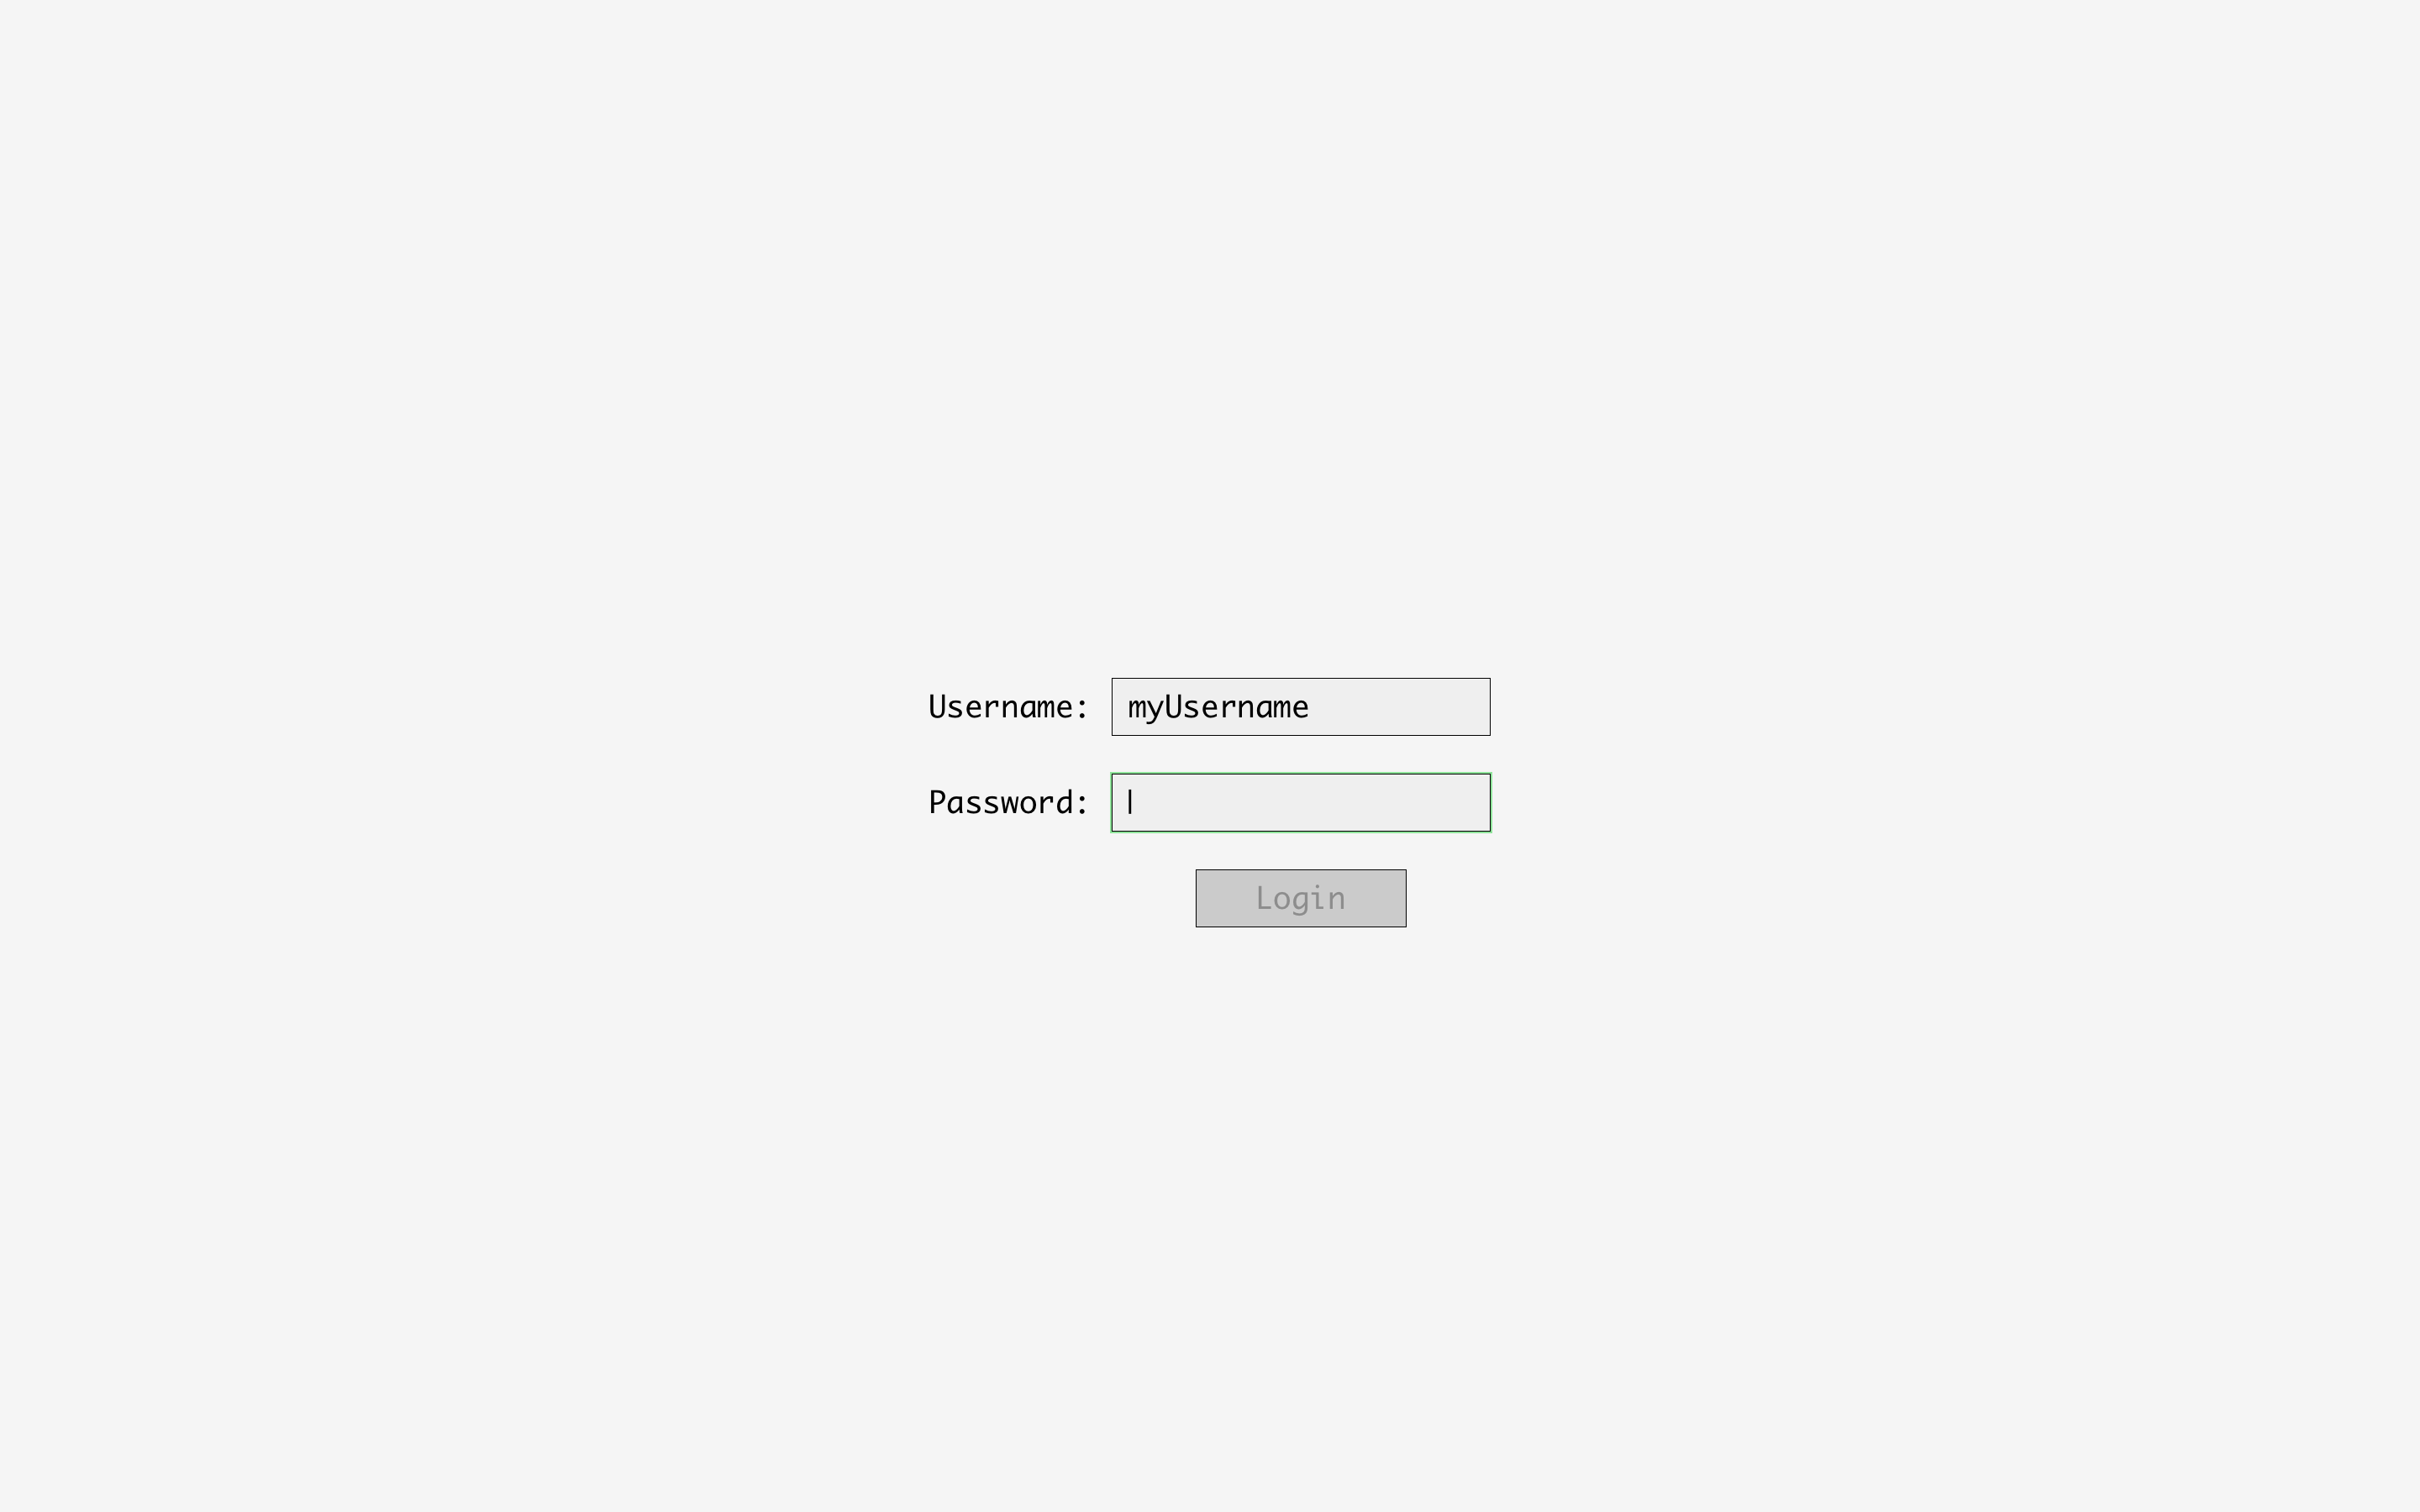
\includegraphics[scale=0.14]{textures/images/annexes/maquettes/1-Login.png}
    \caption{La page d'accueil}
\end{figure}
\begin{figure}[!h]
    \centering
    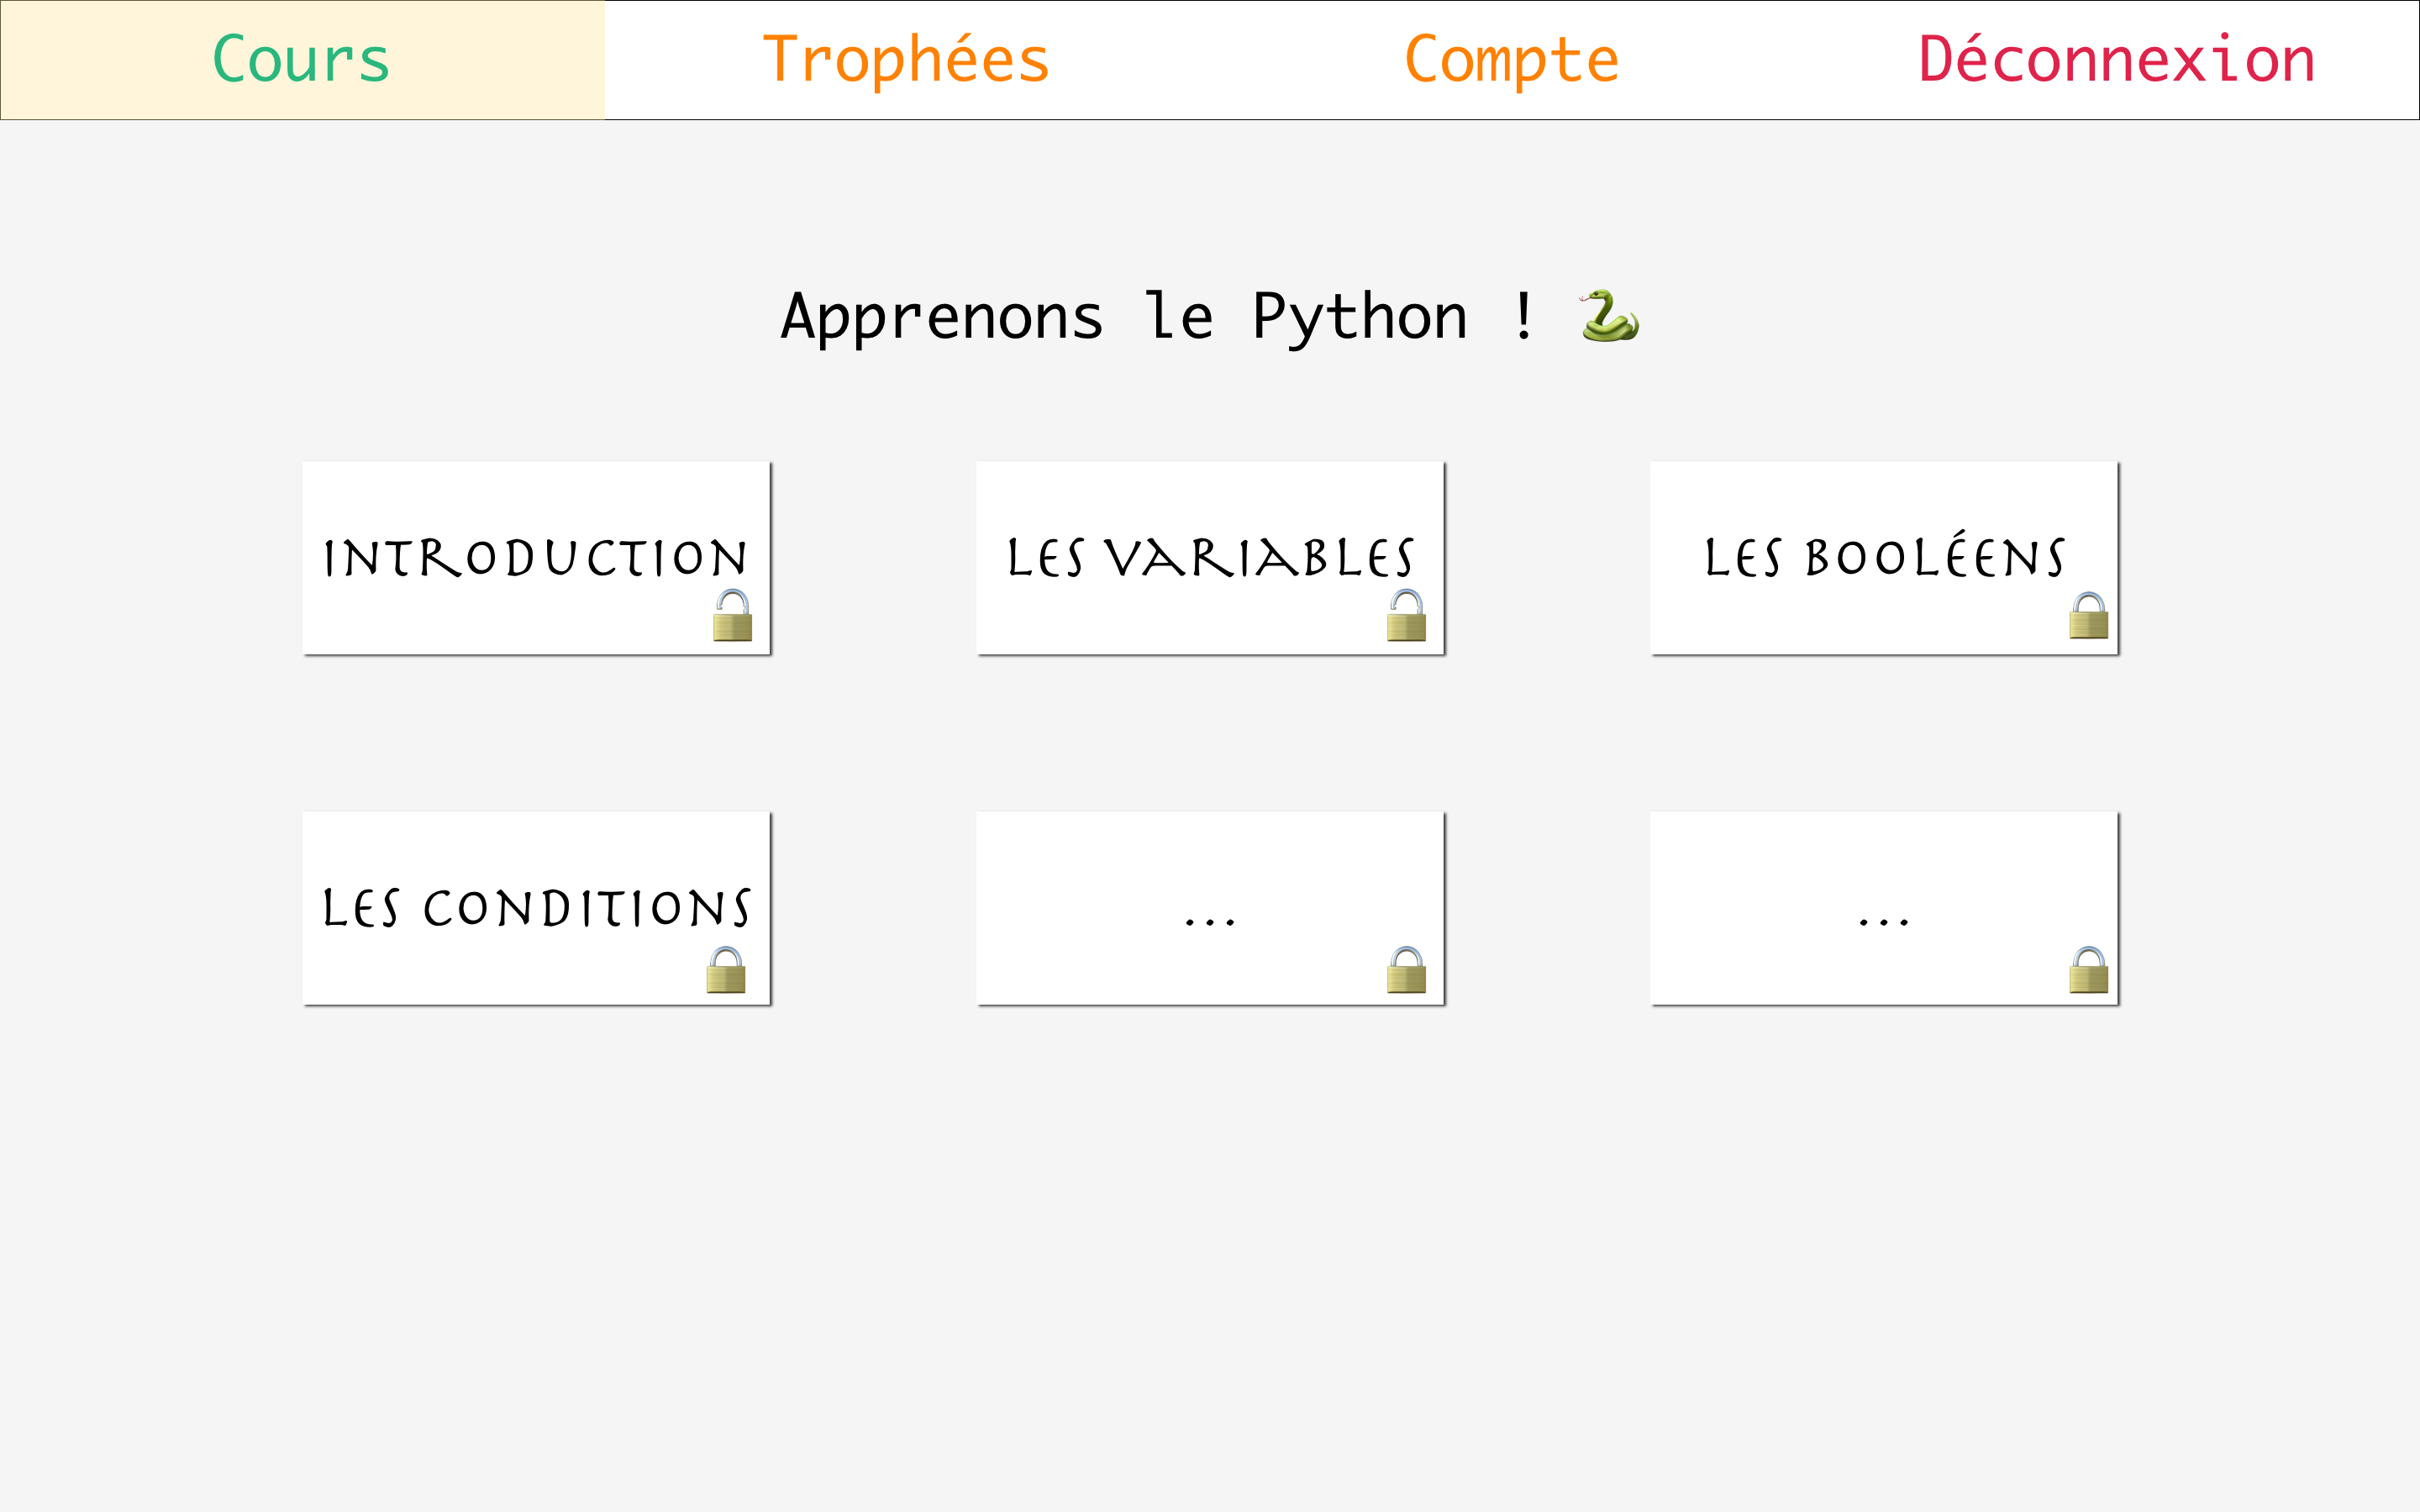
\includegraphics[scale=0.14]{textures/images/annexes/maquettes/21-Sommaire.png}
    \caption{La page de cours}
\end{figure}

\newpage

\begin{figure}[!h]
    \centering
    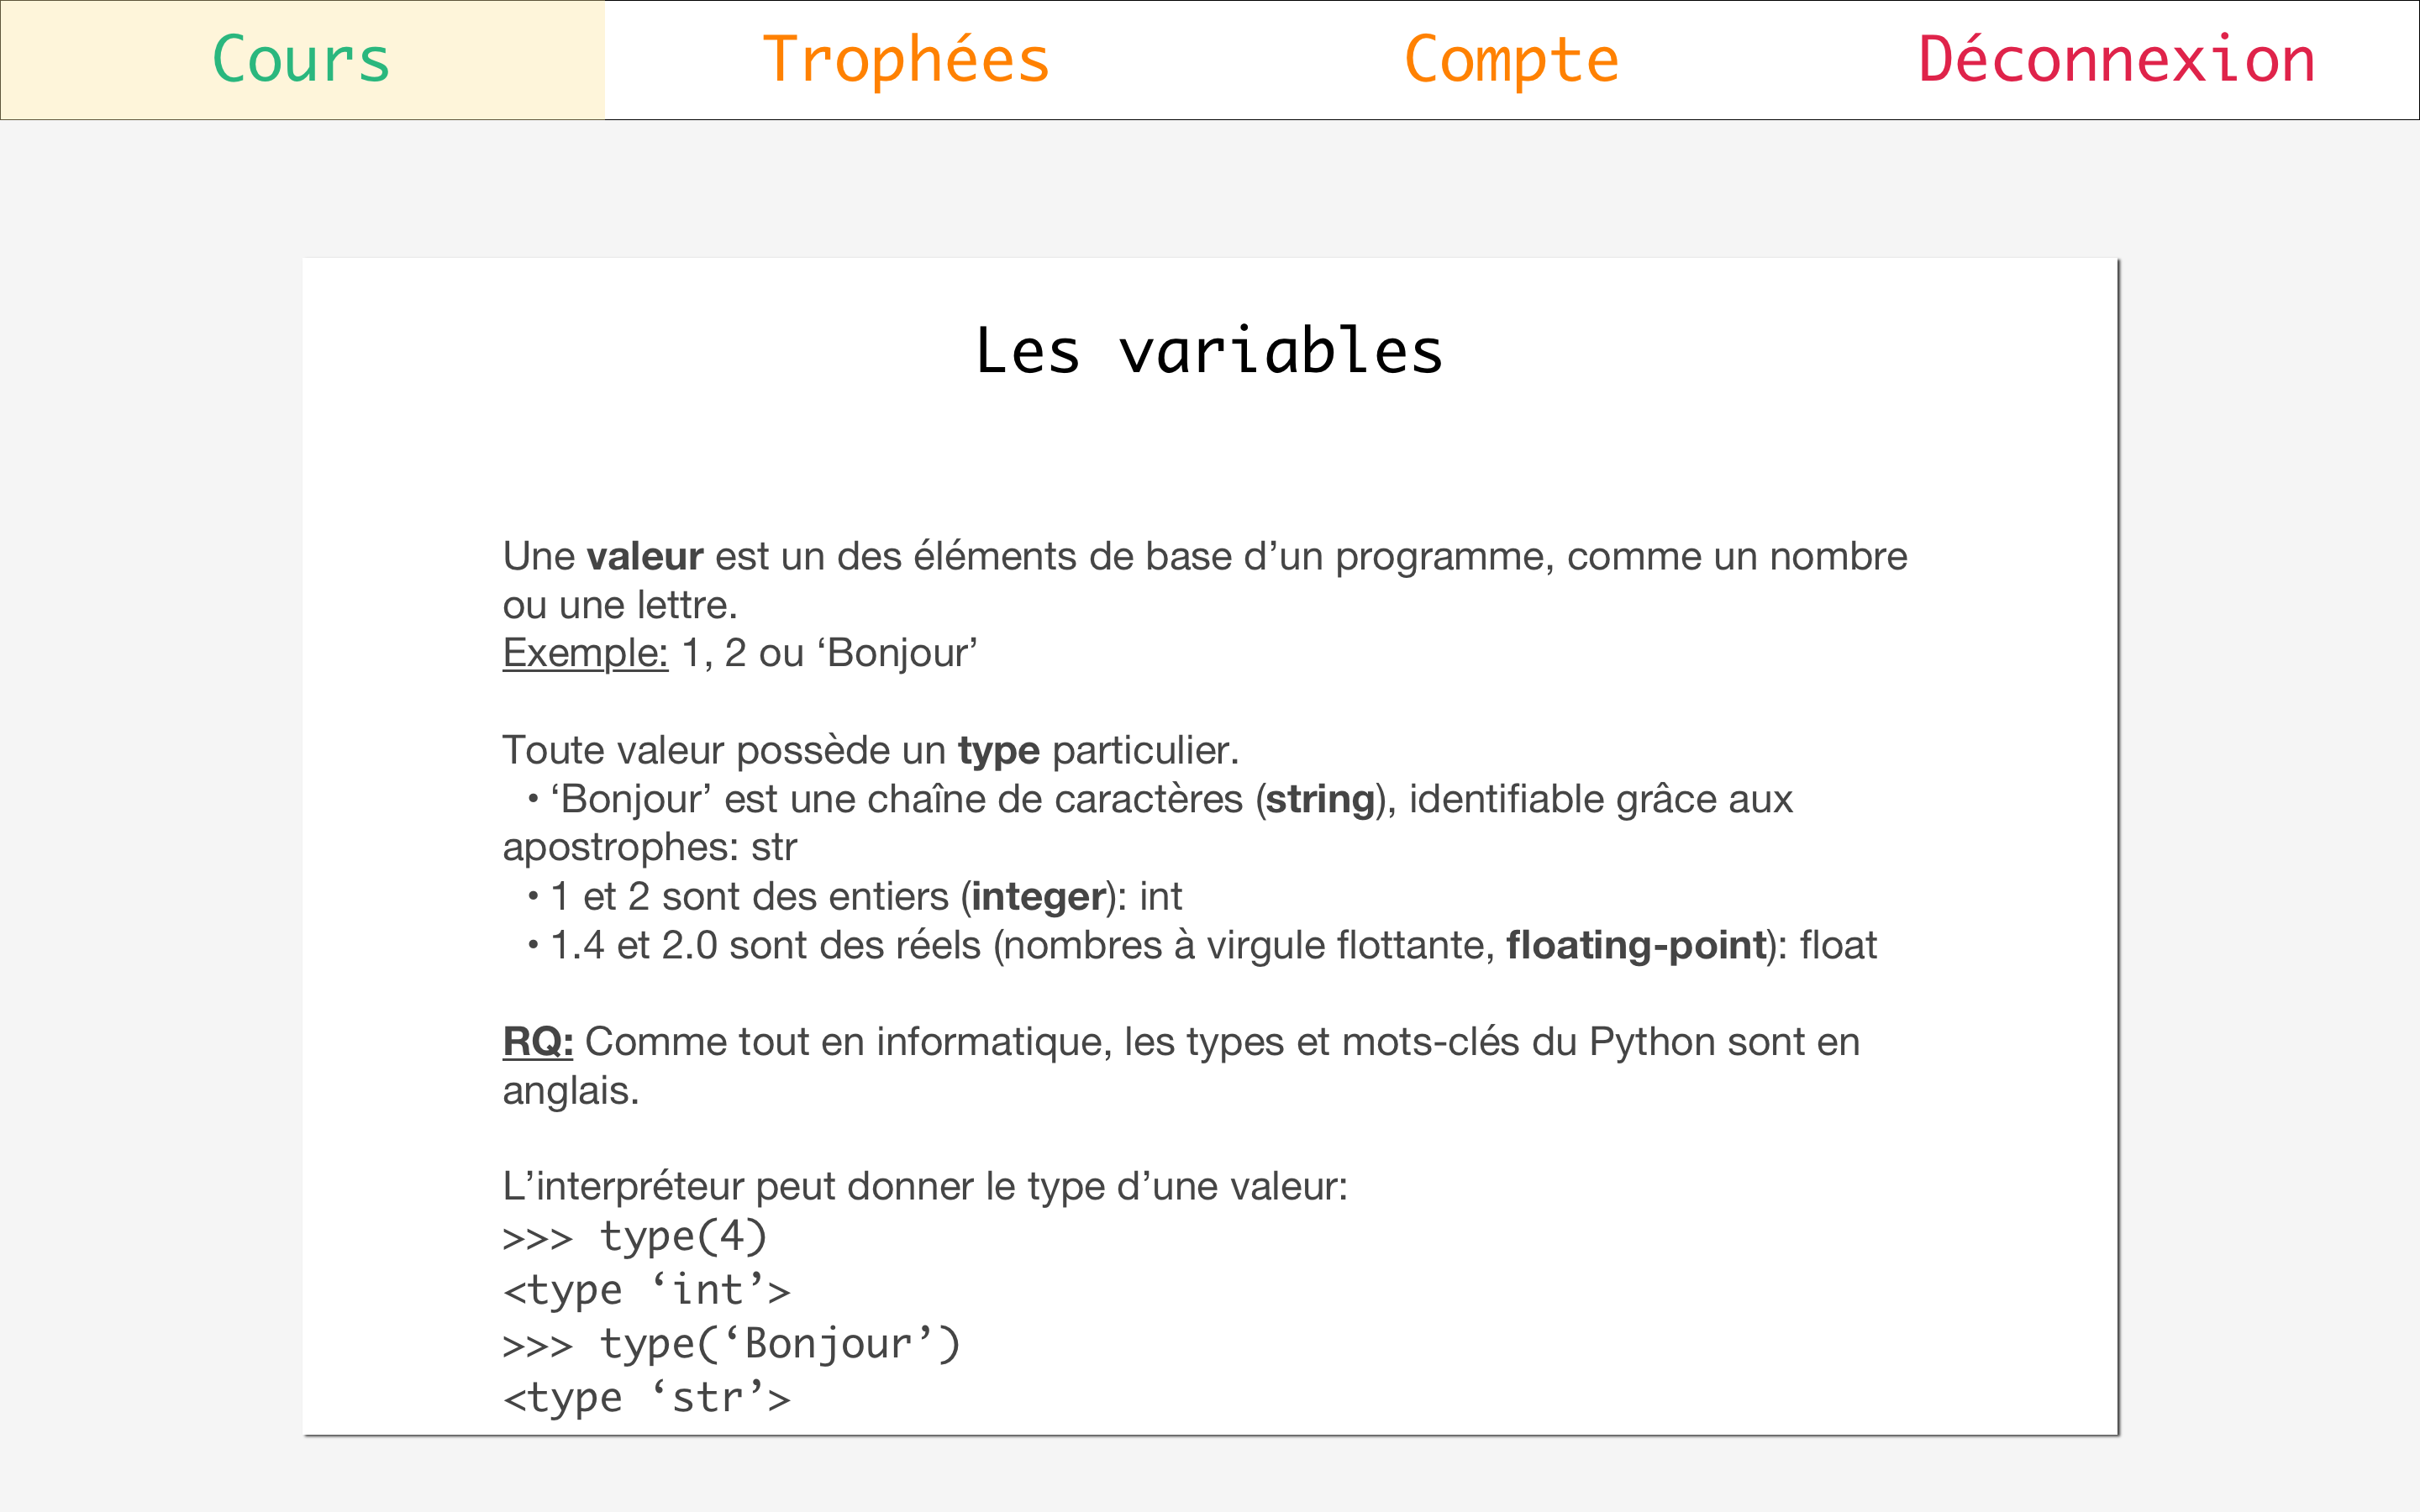
\includegraphics[scale=0.14]{textures/images/annexes/maquettes/22-Cours.png}
    \caption{L'aperçu d'un chapitre}
\end{figure}
\begin{figure}[!h]
    \centering
    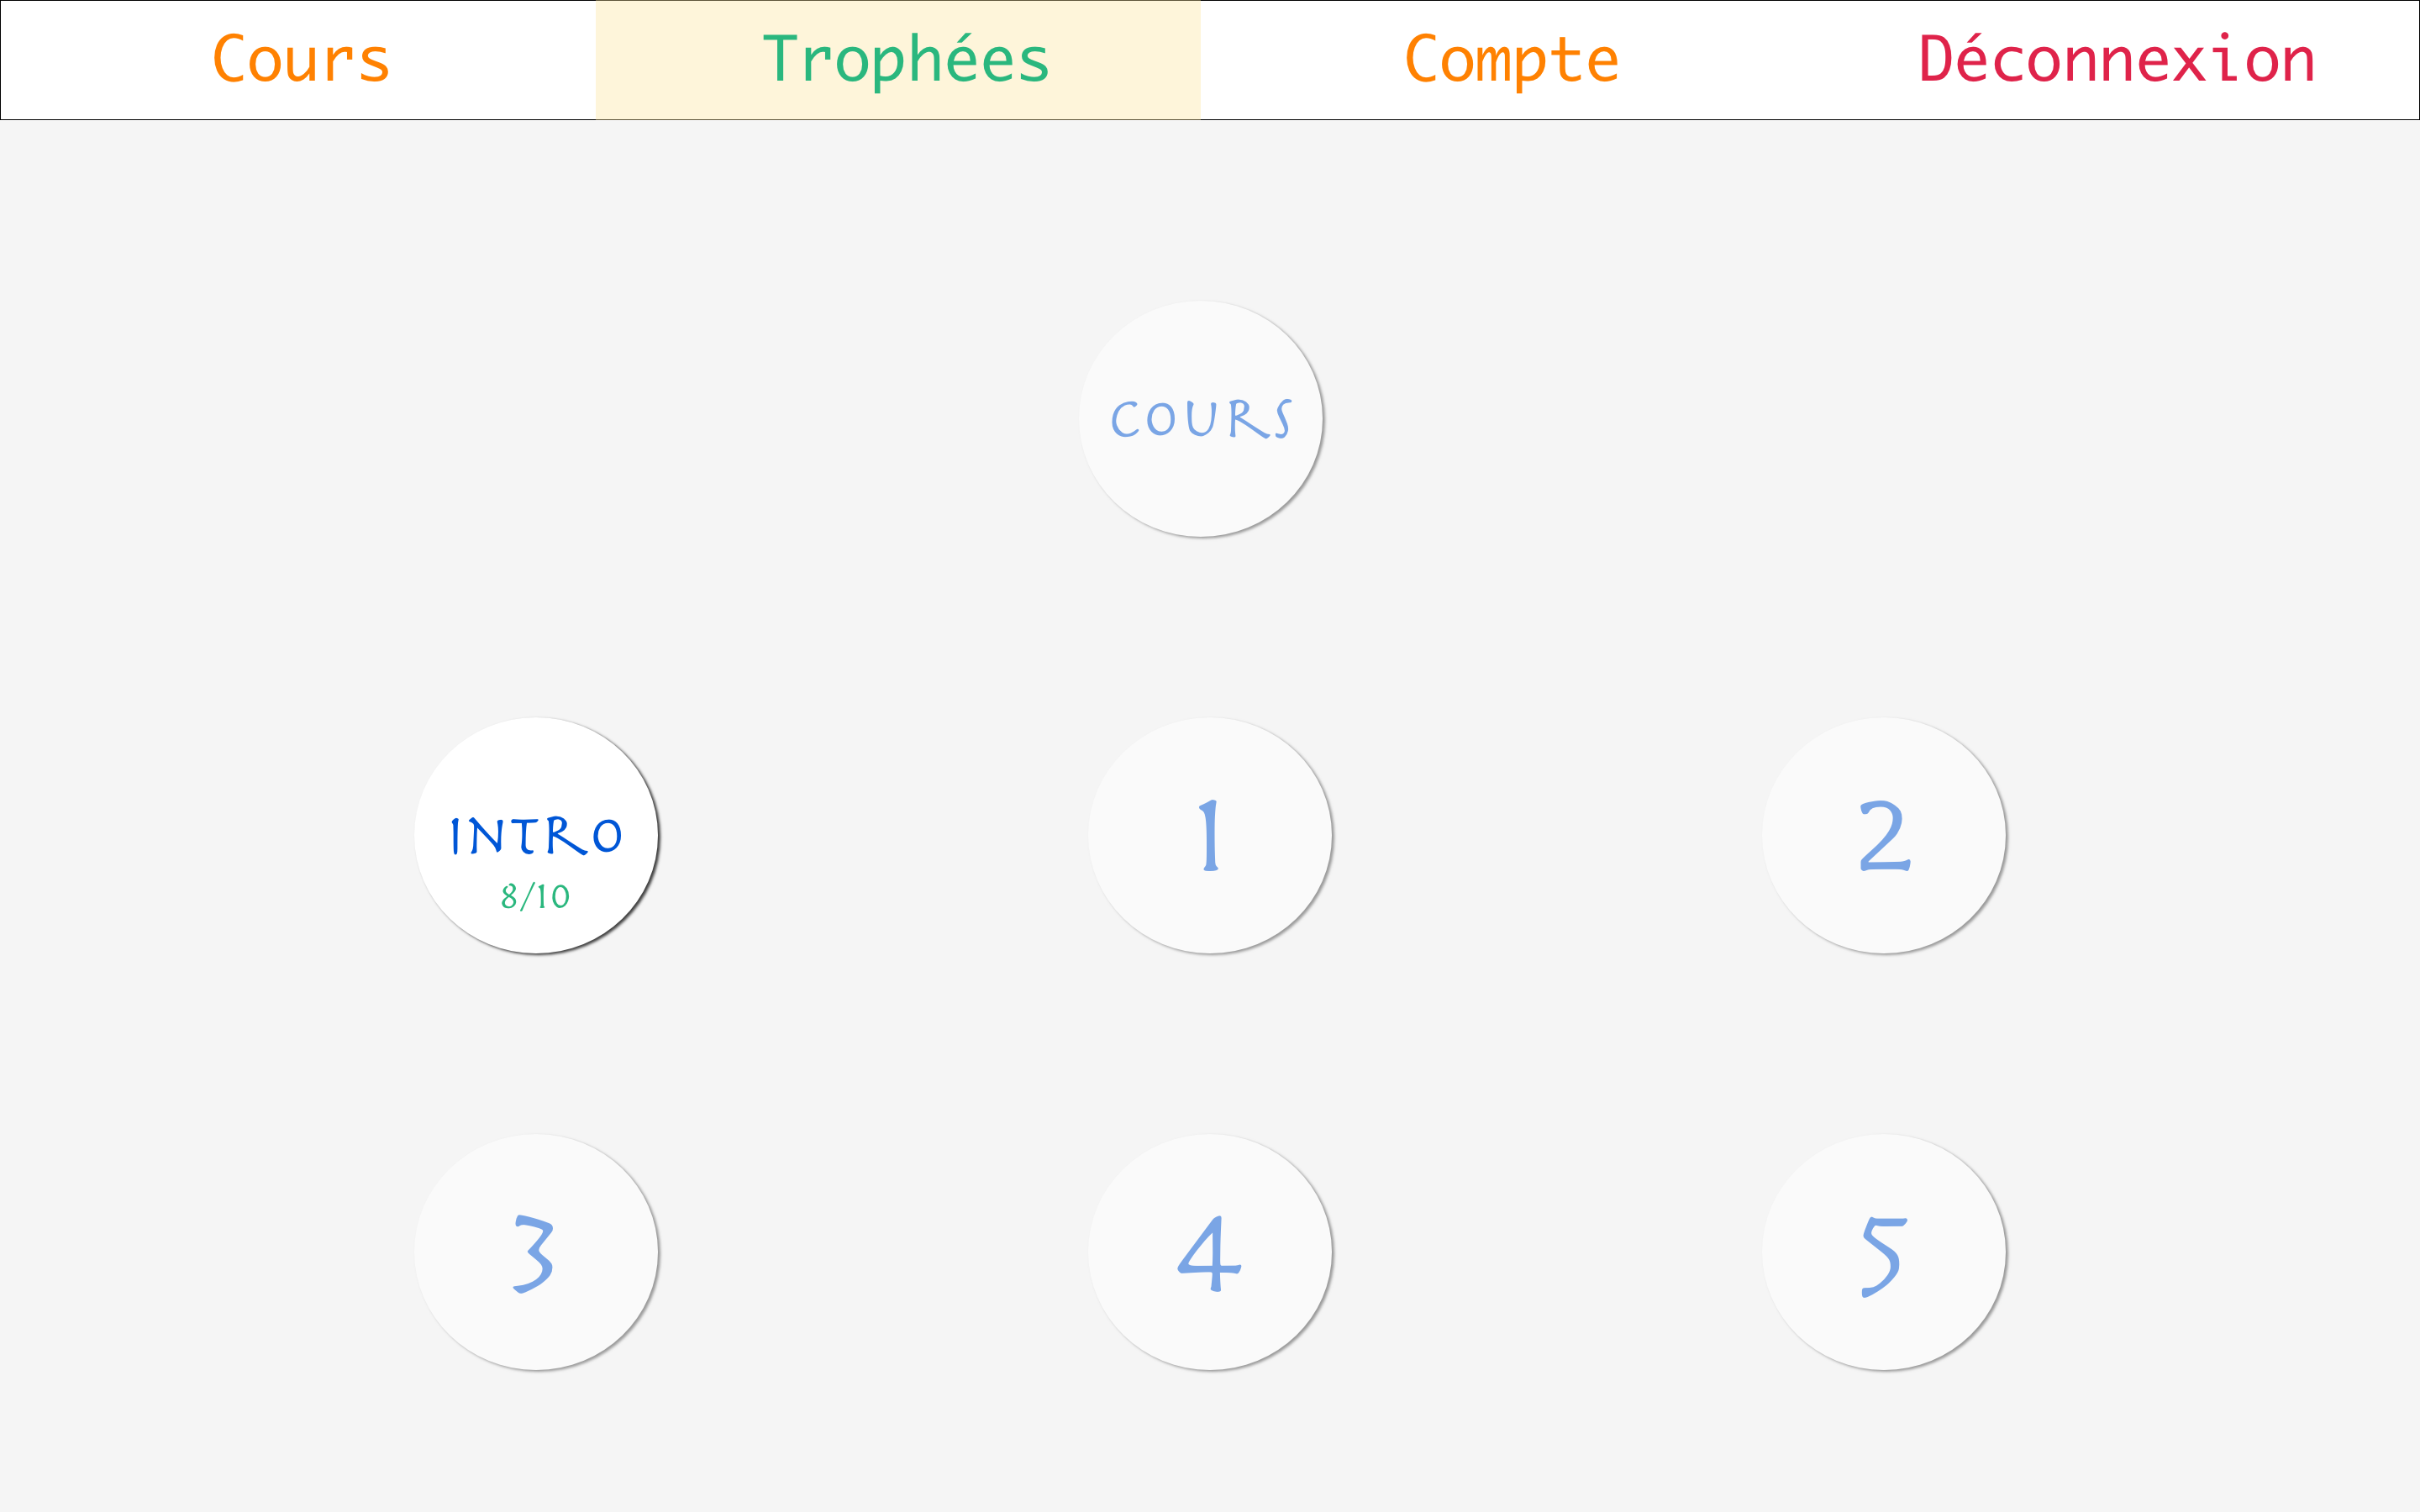
\includegraphics[scale=0.14]{textures/images/annexes/maquettes/3-Trophees.png}
    \caption{La page des trophées}
\end{figure}

\newpage

\begin{figure}[!h]
    \centering
    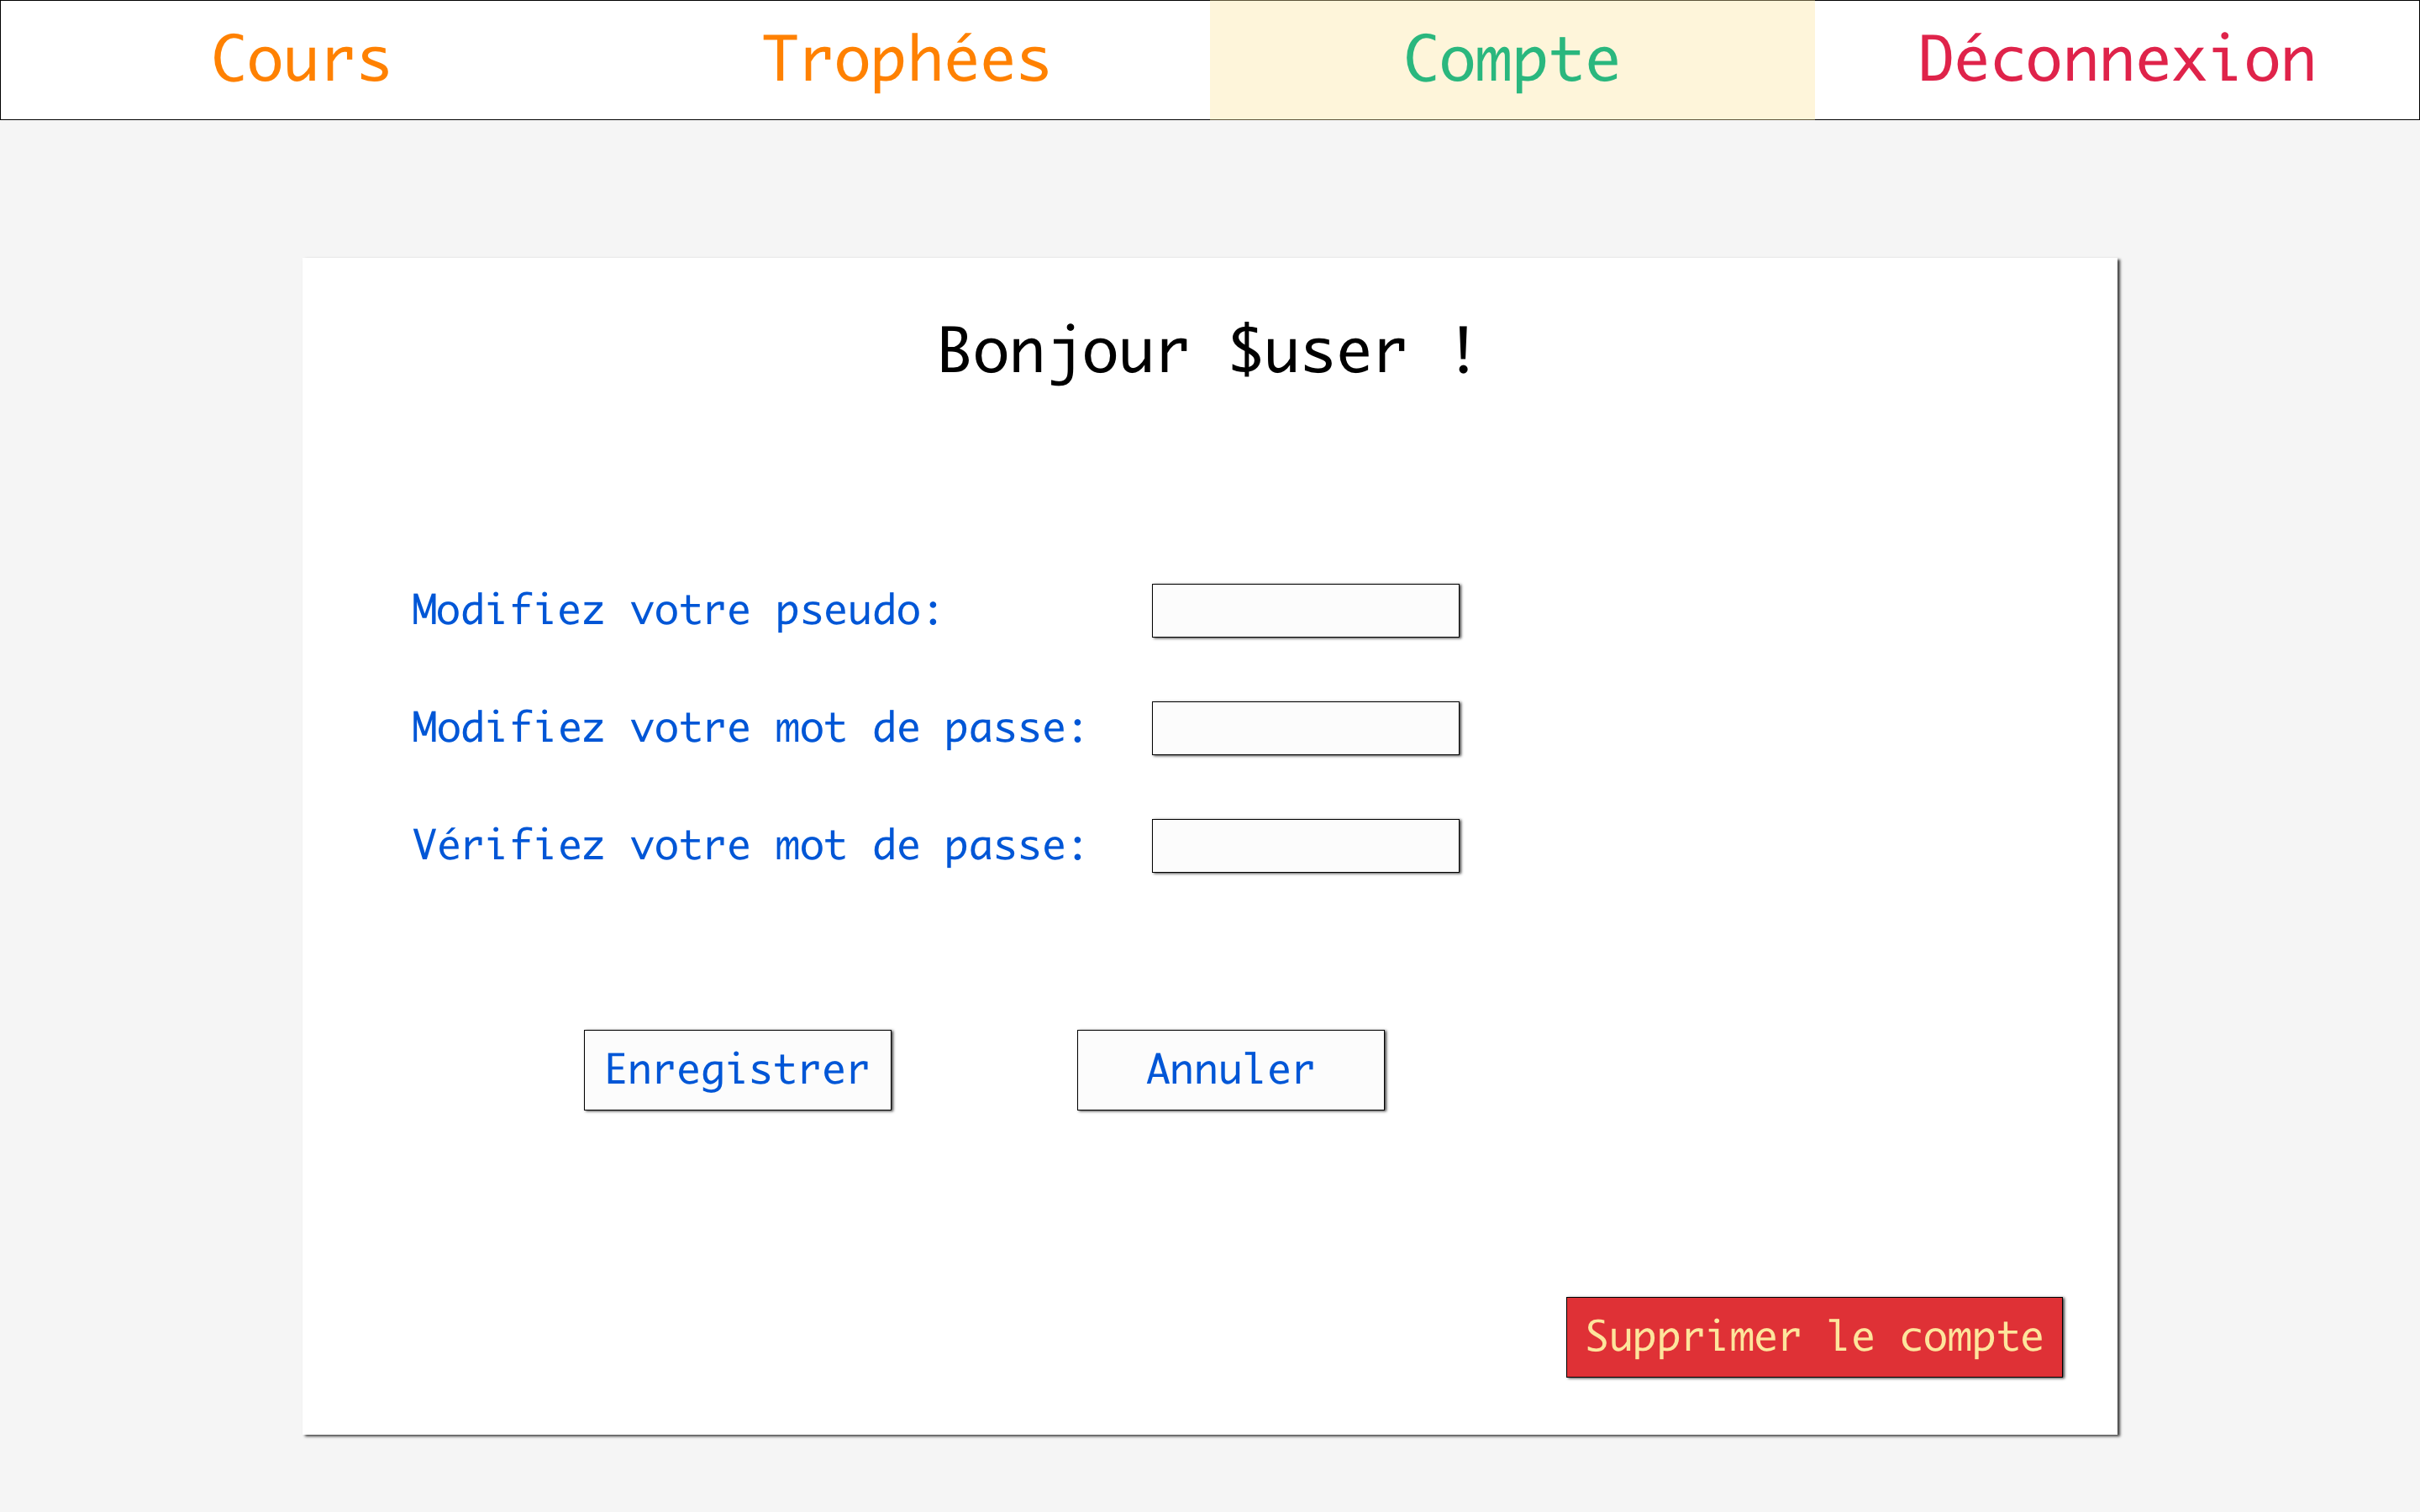
\includegraphics[scale=0.14]{textures/images/annexes/maquettes/4-Compte.png}
    \caption{La page du compte}
\end{figure}
\newpage
\section*{Le site}
\addcontentsline{ptc}{section}{Le site}
\label{sec:site}

Voici les différentes pages du site finalisé :

\begin{figure}[!h]
    \centering
    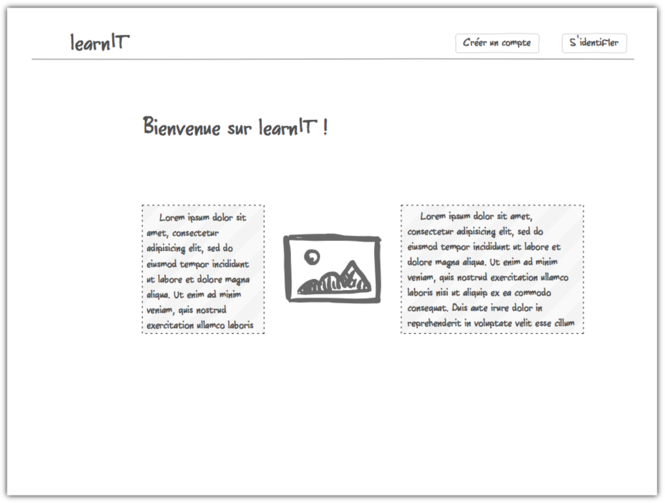
\includegraphics[scale=1]{textures/images/annexes/site/1a-Home.png}
    \caption{La page d'accueil}
\end{figure}
\begin{figure}[!h]
    \centering
    \includegraphics[scale=1]{textures/images/annexes/site/1b-CréerCompte.png}
    \caption{La page d'inscription}
\end{figure}

\newpage

\begin{figure}[!h]
    \centering
    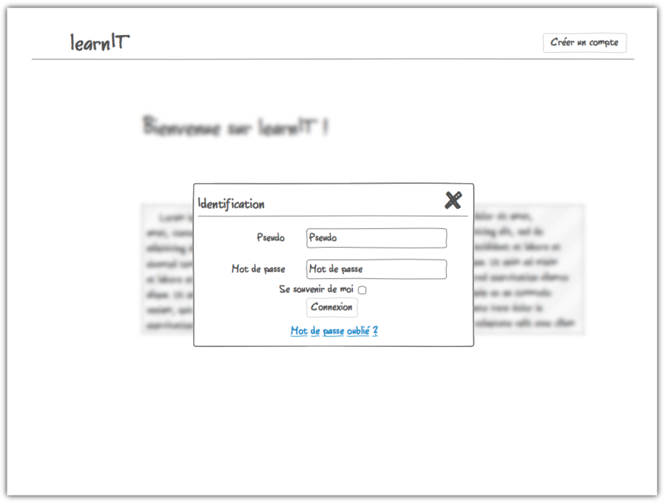
\includegraphics[scale=1]{textures/images/annexes/site/1c-Sidentifier.png}
    \caption{La page de connexion}
\end{figure}
\begin{figure}[!h]
    \centering
    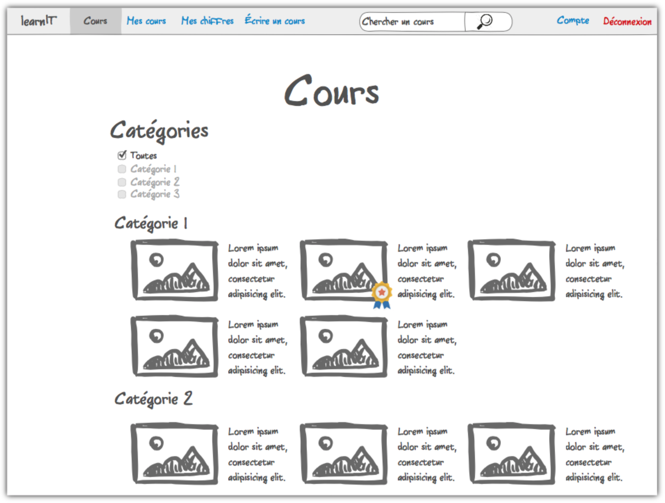
\includegraphics[scale=1]{textures/images/annexes/site/2-Cours.png}
    \caption{La liste des cours}
\end{figure}

\newpage

\begin{figure}[!h]
    \centering
    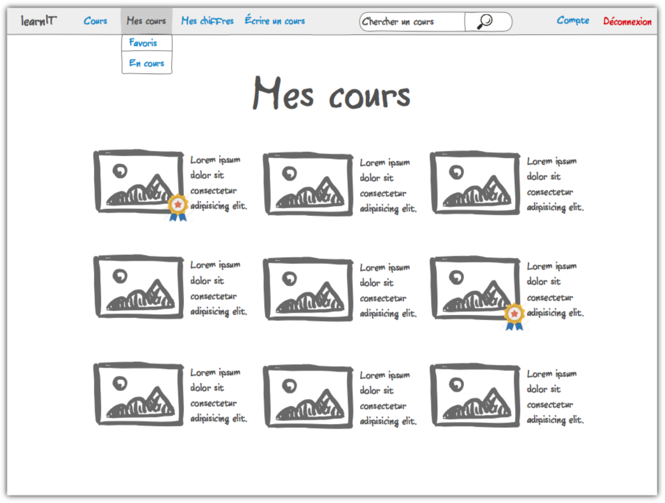
\includegraphics[scale=1]{textures/images/annexes/site/3-MesCours.png}
    \caption{La liste des cours auxquels l'utilisateur est inscrit}
\end{figure}
\begin{figure}[!h]
    \centering
    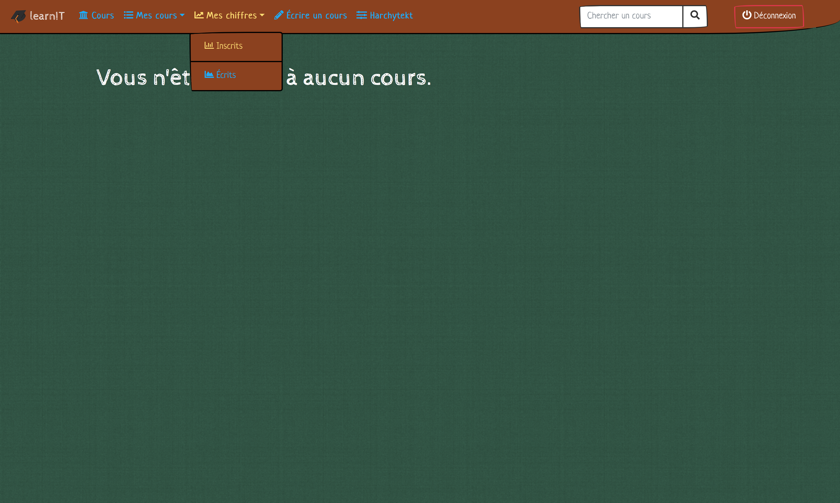
\includegraphics[scale=1]{textures/images/annexes/site/4-MesChiffres(Cours).png}
    \caption{La page des chiffres}
\end{figure}

\newpage

\begin{figure}[!h]
    \centering
    \includegraphics[scale=1]{textures/images/annexes/site/5-ÉcrireCours.png}
    \caption{La page de création d'un cours}
\end{figure}
\begin{figure}[!h]
    \centering
    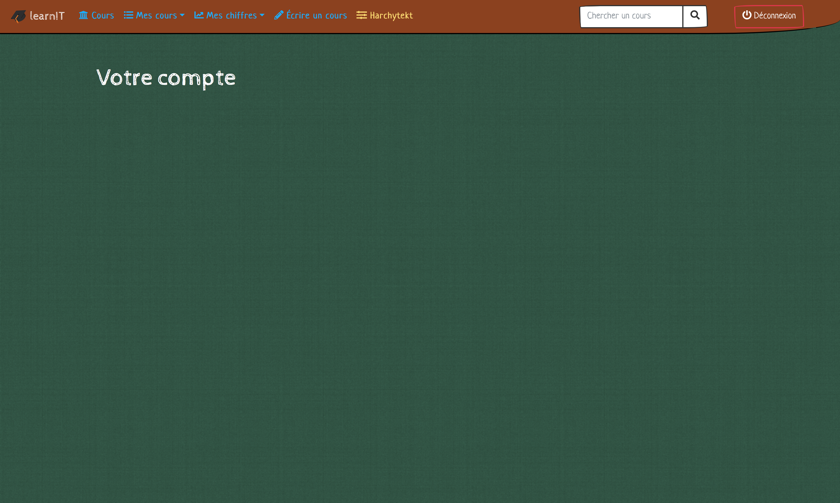
\includegraphics[scale=1]{textures/images/annexes/site/6-Compte(utilisateur).png}
    \caption{La page du compte utilisateur}
\end{figure}

%%% Local Variables:
%%% mode: latex
%%% TeX-master: t
%%% End:
    \newpage
    \newpage
\thispagestyle{empty}
\setcounter{page}{0}
\null
\newpage
\end{document}
